%% =====================================================================
%% HCAN-CIB manuscript -- Elsevier CAS single-column (cas-sc)
%% Needs cas-sc.cls and cas-common.sty in the project (use Overleaf's
%% "Elsevier CAS Single Column" template and replace its main .tex with this).
%% =====================================================================
\documentclass[a4paper,fleqn]{cas-sc}
\usepackage{cmap}
\usepackage[T1]{fontenc}
\usepackage[utf8]{inputenc}

\usepackage[numbers]{natbib}

\usepackage{amsmath,amssymb,amsfonts,bm}
\usepackage{booktabs,array,multirow}
\usepackage{xcolor}
\usepackage{tikz}
\usetikzlibrary{positioning,arrows.meta,calc}
\usepackage{algorithm}
\usepackage{algpseudocode}
\usepackage{url}
\usepackage[section]{placeins}

\graphicspath{{figures/}}
\newcommand{\vrf}[1]{\textcolor{red}{[verify: #1]}}
\newcommand{\pmsd}[2]{$#1\pm#2$}
\DeclareMathOperator{\softmax}{softmax}
\DeclareMathOperator{\Var}{Var}
\DeclareMathOperator{\AUROC}{AUROC}
\newtheorem{proposition}{Proposition}
\newproof{pf}{Proof}

\begin{document}
\let\WriteBookmarks\relax
\def\floatpagefraction{0.8}
\def\textpagefraction{0.001}
\setcounter{topnumber}{4}
\setcounter{bottomnumber}{4}
\setcounter{totalnumber}{8}
\renewcommand{\topfraction}{0.95}
\renewcommand{\bottomfraction}{0.95}
\renewcommand{\textfraction}{0.02}

\shorttitle{Invariance-gated multimodal emotion recognition under LOSO}
\shortauthors{First Author et al.}



\title [mode = title]{Resolving Modality Starvation and Latent Class Collapse in Cross-Subject Multimodal Emotion Recognition: A Hierarchical Invariance-Gated Architecture}

\author[1]{First Author}[orcid=0000-0000-0000-0000]
\cormark[1]
\ead{first.author@university.edu}
\credit{Conceptualization, Methodology, Software, Formal analysis, Writing -- original draft}

\author[1]{Second Author}
\credit{Methodology, Validation, Writing -- review \& editing}

\author[1]{Supervisor Name}
\credit{Supervision, Writing -- review \& editing}

\affiliation[1]{organization={Department of Computer Science and Engineering, University Name},
  city={City},
  country={Country}}

\cortext[cor1]{Corresponding author}

\begin{abstract}
Emotion recognition from electroencephalography (EEG) and peripheral physiology is routinely reported at 75--85\% accuracy, yet most of those figures come from evaluation protocols in which windows of a single recording appear on both sides of the train/test boundary. Under a strict, leakage-free leave-one-subject-out (LOSO) protocol the picture changes sharply: three widely used deep baselines (EEGNet, ACRNN, a plain 1D-CNN) land between 0.49 and 0.54 AUROC on both DEAP (32 subjects) and DREAMER (23 subjects). We trace this failure to three interacting causes: biased, majority-leaning predictions at the level of individual held-out subjects, gradient starvation between modalities and channels, and an inter-subject variance that is $349.6\times$ larger than the emotion-label variance in DEAP differential-entropy features. Diagnostic probing reveals an extreme $19\times$--$30\times$ gradient imbalance; yet across 1,152 trained models on DEAP, off-the-shelf gradient modulation techniques (OGM-GE, UDI, PCGrad) fail to improve cross-subject generalization because they treat EEG as a monolithic block and amplify non-invariant channels. This motivates HCAN-CIB, a Hierarchical Cross-Attention Network with Channel and Modality Invariance Balancing. It combines per-channel temporal encoders, region-grouped fusion with an L2 spectral-decoupling penalty, an EMA-driven invariance gate that re-weights cortical regions by their cross-subject stability, transductive per-subject Z-scoring, and latent-space minority oversampling (systematically evaluating V-SMOTE, GAMO, and DeepSMOTE). On DREAMER, the full pipeline moves AUROC from $0.4783\pm0.1395$ (base HCAN-CIB) to $0.5381\pm0.1567$ with Z-scoring and to $0.5589\pm0.1638$ with DeepSMOTE, turning the Gini coefficient positive ($+0.1178$) and lowering expected calibration error to $0.2249$. Across the latent oversampling family, distinct strengths emerge: GAMO achieves the highest balanced accuracy ($0.5167\pm0.1003$), PR-AUC ($0.5237\pm0.1501$), MCC ($0.0398\pm0.2049$), and minority recall ($0.6385\pm0.4010$) among all evaluated pipelines; V-SMOTE achieves peak raw accuracy on DREAMER ($0.5604\pm0.1380$) and leads DEAP minority recall ($0.5404\pm0.2244$), eliminating majority collapse; while DeepSMOTE maximizes discriminative AUROC and probability calibration. Yet, on DEAP a shallow logistic regression on Z-scored differential-entropy features still reaches $0.5754\pm0.0991$ AUROC and outperforms every deep model. Diagnostics show that learned embeddings remain organised by subject rather than by emotion. We therefore position inter-subject domain shift, not class imbalance or modality imbalance, as the remaining bottleneck, and we release a leakage-free benchmark across 55 subjects as a reference point for future work.
\end{abstract}

\begin{keywords}
Emotion recognition \sep EEG \sep multimodal fusion \sep leave-one-subject-out \sep gradient starvation \sep spectral decoupling \sep latent minority oversampling \sep GAMO \sep DeepSMOTE \sep domain shift
\end{keywords}

\maketitle

\section{Introduction}
\label{sec:intro}

Affective computing aims to infer a person's emotional state from signals the person does not consciously control. Scalp EEG reflects cortical activity that is directly tied to appraisal and valence processing, while peripheral channels such as electrocardiography (ECG), galvanic skin response, and respiration capture the autonomic side of the same episode. Combining the two is attractive because each modality is partially blind where the other is informative: autonomic signals respond slowly and non-specifically, whereas EEG is fast but dominated by noise and by anatomy.

A usable system must work on a person it has never seen. That requirement makes leave-one-subject-out (LOSO) validation the only protocol with clinical meaning: every trial, window, and normalisation statistic that touches the held-out person must be excluded from training and model selection. Many published pipelines do not satisfy this requirement. Random splits over overlapping windows, or subject-dependent 10-fold schemes, allow the network to see near-duplicates of test segments during training, and the reported accuracy then measures memorisation of a recording rather than recognition of an emotion \citep{li2022tutorial}.

We build a strictly leakage-free LOSO pipeline for DEAP \citep{koelstra2012deap} and DREAMER \citep{katsigiannis2018dreamer}, incorporating recent benchmark standardization recommendations \citep{torres2023survey,zhang2023multimodal}, and ask why deep multimodal models fail under it. Our experiments isolate three obstacles.

\begin{enumerate}
\item \textbf{Biased predictions at the subject level.} Each person uses the rating scale differently, so the binary labels of a held-out subject can be skewed, and models that minimise cross-entropy drift toward the more frequent class. On DEAP, EEGNet predicts the minority class for only $29.1\%$ of windows; its Macro-F1 is $0.4005$.
\item \textbf{Modality and channel starvation.} When a high-dimensional EEG stream is fused with a low-dimensional peripheral vector, the branch with the steeper initial loss descent captures the gradient budget and the other branch is barely trained \citep{pezeshki2021gradient,huang2022modality,fan2023pmr}. We show through diagnostic probing that the joint network suffers a $19\times$--$30\times$ gradient imbalance, and we demonstrate across 1,152 trained models that existing gradient modulation methods (such as OGM-GE and UDI) fail because they treat EEG as a monolithic block rather than isolating invariant cortical regions.
\item \textbf{Inter-subject variance.} In DEAP differential-entropy (DE) features, subject identity explains $47.75\%$ of the variance and the emotion label explains $0.137\%$, a ratio of $349.6{:}1$. Subject identity can be decoded with $97.81\%$ accuracy, against a chance level of $3.125\%$.
\end{enumerate}

Our contributions are as follows.
\begin{itemize}
\item We provide an empirical investigation of modality starvation in multimodal EEG-physiological computing across 1,152 trained models on DEAP, showing that off-the-shelf gradient modulation techniques (OGM-GE, UDI, PCGrad) fail because they blindly amplify noisy, non-generalizing cortical channels.
\item Motivated by these findings, we propose HCAN-CIB, which transitions from modality-level damping to channel-level invariance filtering by combining channel-independent 1D feature extraction, region-grouped spectral decoupling, and an EMA-based invariance gate that re-weights cortical regions according to their cross-subject stability.
\item We integrate and systematically benchmark latent-space minority oversampling (evaluating V-SMOTE, GAMO, and DeepSMOTE) within the multimodal fused embedding, averting the corruption of artifact-laden raw EEG time series while rescuing minority recall from severe majority-class collapse.
\item We report a leakage-free benchmark over 55 subjects (32 DEAP and 23 DREAMER) with paired non-parametric tests, calibration metrics, and interpretability analyses, including a negative result: a shallow linear model on normalised DE features beats all deep models on DEAP.
\end{itemize}

The rest of the paper is organised as follows. Section~\ref{sec:related} reviews related work, Section~\ref{sec:method} presents HCAN-CIB, Section~\ref{sec:setup} describes the experimental protocol, Section~\ref{sec:results} reports and discusses results, and Section~\ref{sec:conclusion} concludes.

%% ---------------------------------------------------------------------
\section{Literature Survey}
\label{sec:related}

\subsection{Deep architectures for EEG emotion recognition}
Compact convolutional networks and hybrid attention models dominate current practice. EEGNet couples temporal convolutions with depthwise spatial filters \citep{lawhern2018eegnet}, while recent conformer and transformer architectures capture global oscillatory dependencies \citep{song2023conformer}. ACRNN adds channel-wise attention and self-attention on top of a convolutional--recurrent stack and reports strong results on DEAP \citep{tao2020acrnn}. Most modern pipelines bypass raw waveforms entirely, extracting band-limited differential entropy (DE) features \citep{liu2022comparing,lu2023cross} that discard high-frequency phase information. A recent review catalogues these designs and highlights the heterogeneity of evaluation protocols across papers \citep{li2022tutorial}. A shared design choice in the convolutional models is early spatial mixing: the depthwise spatial kernel collapses all electrodes into a handful of virtual channels before any region-specific structure is learned.

\subsection{Multimodal fusion and gradient starvation}
Joint training of several modalities frequently underperforms the best unimodal model, because the branches overfit and generalise at different rates \citep{huang2022modality,zhou2023modality}. Subsequent work attributes the effect to modality competition and proposes on-the-fly gradient modulation or prototypical rebalancing to slow the dominant branch \citep{peng2022balanced,fan2023pmr}. Gradient starvation provides a more general account: once a feature allows the loss to fall quickly, the gradient signal for slower features shrinks toward zero. Spectral decoupling, a penalty on the magnitude of the network output, counteracts this effect by keeping the loss from saturating on the dominant feature \citep{pezeshki2021gradient}. We adapt that idea to intermediate representations and make it region-aware.

\subsection{Class imbalance and domain adaptation in physiological computing}
SMOTE interpolates between minority neighbours in input space \citep{elreedy2021smote}, which is hazardous for raw EEG because linear blends of two waveforms generally do not resemble real brain activity. Generative approaches such as GAMO operate on learned features \citep{mullick2019gamo}, and DeepSMOTE performs SMOTE-style interpolation inside the latent space of an autoencoder \citep{dablain2023deepsmote}. For subject shift, domain-adversarial and domain-generalization training remove domain identity from the features through invariant feature learning \citep{wang2023cross}, and bi-hemispheric adversarial variants have been applied to EEG emotion recognition \citep{li2021bidann}.

\subsection{Gap}
Three observations motivate this work. First, evaluation protocols that leak windows across the split inflate reported accuracy. Second, imbalance remedies and modality-balancing remedies are usually proposed and evaluated separately, so their individual contributions to cross-subject performance remain confounded. Third, the effect of subject-level amplitude offsets is seldom quantified. Our study evaluates all three factors under one leakage-free protocol and with matched metrics.

%% ---------------------------------------------------------------------
\section{Methodology}
\label{sec:method}

\subsection{Problem statement}
Let $\mathcal{D}=\{\mathcal{S}_1,\dots,\mathcal{S}_K\}$ be a collection of $K$ subjects, where $\mathcal{S}_k=\{(\mathbf{X}^{\mathrm{eeg}}_{k,i},\mathbf{X}^{\mathrm{per}}_{k,i},y_{k,i})\}_{i=1}^{n_k}$. Each EEG window satisfies $\mathbf{X}^{\mathrm{eeg}}\in\mathbb{R}^{C\times T}$, with $C$ electrodes and $T$ samples. The peripheral recording $\mathbf{X}^{\mathrm{per}}\in\mathbb{R}^{P\times T'}$ is reduced by a fixed statistical descriptor map to a vector $\mathbf{p}\in\mathbb{R}^{d_p}$ with $d_p=24$ for DEAP and $d_p=12$ for DREAMER. The label $y\in\{0,1\}$ is the binarised valence class. In fold $k$, the model is fitted on $\mathcal{D}\setminus\mathcal{S}_k$ and evaluated only on $\mathcal{S}_k$:
\begin{equation}
\theta_k^\star=\arg\min_{\theta}\;\mathbb{E}_{(\mathbf{X},y)\sim\mathcal{D}\setminus\mathcal{S}_k}\,\ell\bigl(f_\theta(\mathbf{X}),y\bigr),\qquad
\text{score}_k=M\bigl(f_{\theta_k^\star},\mathcal{S}_k\bigr).
\end{equation}

\subsection{Transductive per-subject Z-scoring}
Scalp impedance, skull thickness, and resting alpha power shift the amplitude distribution of every person. For subject $s$, channel $c$, we compute the mean $\mu_{s,c}$ and standard deviation $\sigma_{s,c}$ over all samples of that subject's recording and set
\begin{equation}
\tilde{x}_{s,c,t}=\frac{x_{s,c,t}-\mu_{s,c}}{\sigma_{s,c}+10^{-8}}.\label{eq:z}
\end{equation}
The statistics use no labels, but they use the unlabeled recording of the test subject, so the step is transductive. In deployment it requires a short calibration recording of the new user. The same normalisation is applied to the ECG and peripheral inputs.

\subsection{Overview}
Figure~\ref{fig:arch} shows the data flow for DEAP. The EEG branch is processed by channel-independent encoders (Stage~A). Stage~D latent minority oversampling (evaluating V-SMOTE, GAMO, and DeepSMOTE) operates on the extracted channel representations and peripheral descriptors during training only. The augmented channel representations are aggregated into regional tokens by intra-region attention (Stage~C) and re-weighted by the invariance gate (Stage~B). The peripheral branch yields a single query token, cross-modal attention fuses the two streams, and a linear head produces the classification logit.

\begin{figure}[t]
\centering
\resizebox{\textwidth}{!}{%
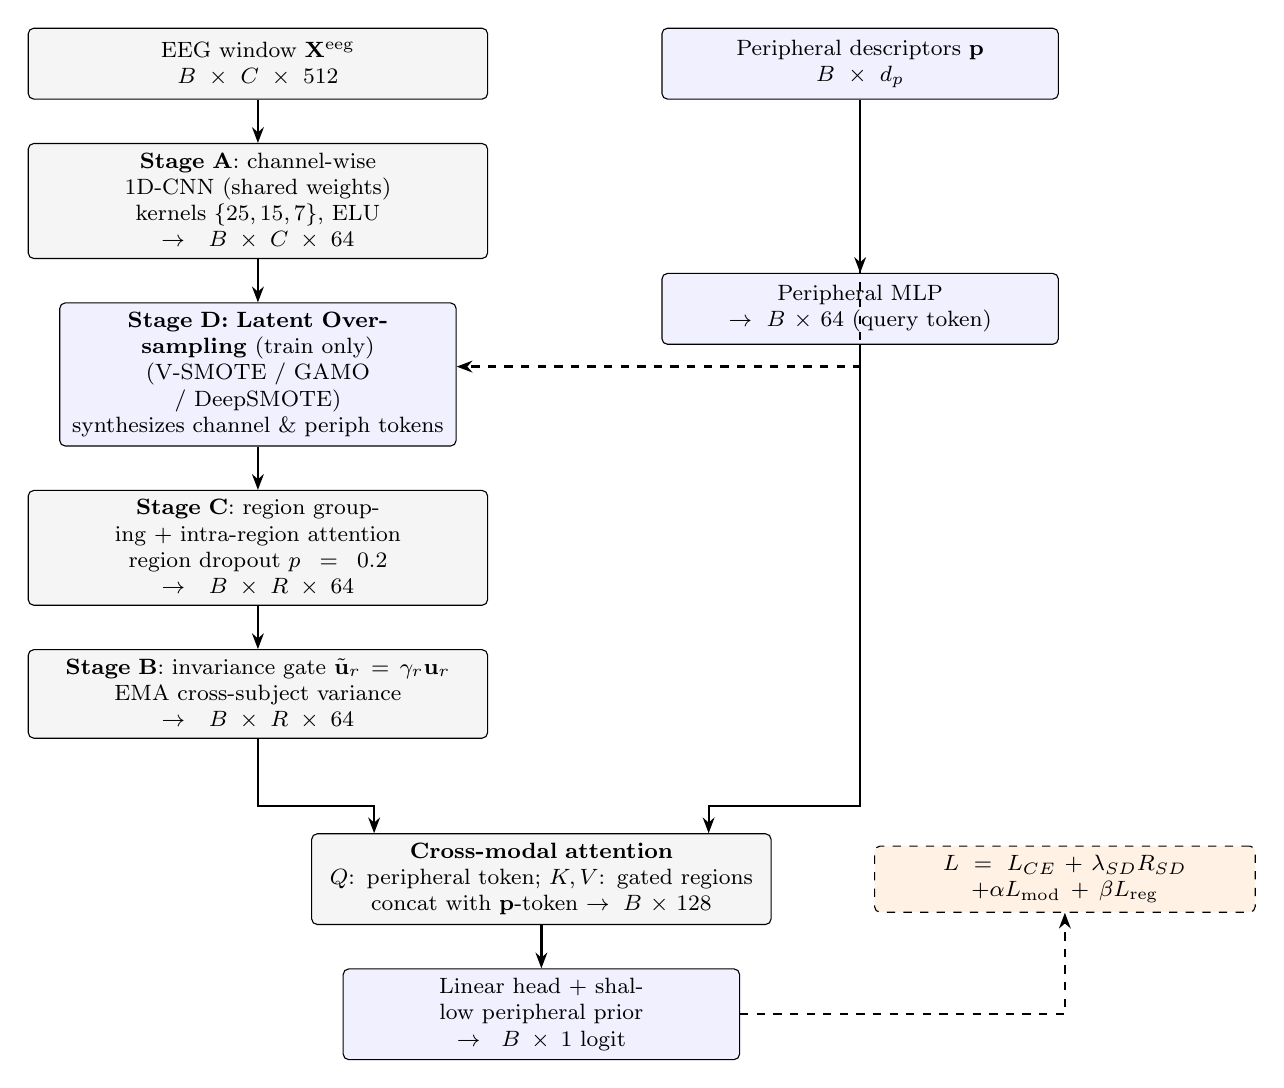
\begin{tikzpicture}[
  node distance=0.55cm,
  blk/.style={draw,rounded corners=2pt,align=center,font=\footnotesize,minimum height=0.9cm,text width=5.6cm,fill=gray!8},
  sm/.style={draw,rounded corners=2pt,align=center,font=\footnotesize,minimum height=0.9cm,text width=4.8cm,fill=blue!6},
  loss/.style={draw,dashed,rounded corners=2pt,align=center,font=\footnotesize,text width=4.6cm,fill=orange!10},
  arr/.style={-{Stealth[length=2mm]},thick}]
\node[blk] (eeg) {EEG window $\mathbf{X}^{\mathrm{eeg}}$\\$B\times C\times 512$};
\node[blk,below=of eeg] (sa) {\textbf{Stage A}: channel-wise 1D-CNN (shared weights)\\kernels $\{25, 15, 7\}$, ELU\\$\to B\times C\times 64$};
\node[sm,below=of sa] (ds) {\textbf{Stage D: Latent Oversampling} (train only)\\(V-SMOTE / GAMO / DeepSMOTE)\\synthesizes channel \& periph tokens};
\node[blk,below=of ds] (sc) {\textbf{Stage C}: region grouping + intra-region attention\\region dropout $p=0.2$\\$\to B\times R\times 64$};
\node[blk,below=of sc] (sb) {\textbf{Stage B}: invariance gate $\tilde{\mathbf{u}}_r=\gamma_r\mathbf{u}_r$\\EMA cross-subject variance\\$\to B\times R\times 64$};
\node[sm,right=2.2cm of eeg] (per) {Peripheral descriptors $\mathbf{p}$\\$B\times d_p$};
\node[sm,below=2.2cm of per] (mlp) {Peripheral MLP\\$\to B\times 64$ (query token)};
\node[blk,below=1.2cm of sb,xshift=3.6cm] (xa) {\textbf{Cross-modal attention}\\$Q$: peripheral token; $K,V$: gated regions\\concat with $\mathbf{p}$-token $\to B\times128$};
\node[sm,below=of xa] (hd) {Linear head $+$ shallow peripheral prior\\$\to B\times1$ logit};
\node[loss,right=1.3cm of xa] (ls) {$L=L_{CE}+\lambda_{SD}R_{SD}$\\$+\alpha L_{\mathrm{mod}}+\beta L_{\mathrm{reg}}$};
\draw[arr] (eeg)--(sa); \draw[arr] (sa)--(ds); \draw[arr] (ds)--(sc); \draw[arr] (sc)--(sb);
\draw[arr] (per)--(mlp);
\draw[arr,dashed] (per.south) |- ($(ds.east)+(0,0.1)$);
\draw[arr] (sb.south) |- ($(xa.north west)+(0.8,0.35)$) -- ($(xa.north west)+(0.8,0)$);
\draw[arr] (mlp.south) |- ($(xa.north east)+(-0.8,0.35)$) -- ($(xa.north east)+(-0.8,0)$);
\draw[arr] (xa)--(hd);
\draw[arr,dashed] (hd.east) -| (ls.south);
\end{tikzpicture}}
\caption{HCAN-CIB data flow for DEAP ($C=32$, $R=5$, $d_p=24$). For DREAMER, $C=14$, $R=4$ and $d_p=12$. $B$ denotes batch size. Dashed elements are training-time only.}
\label{fig:arch}
\end{figure}

\subsection{Stage A: channel-independent temporal encoders}
Standard depthwise spatial convolutions merge all electrodes in a single learned kernel, which couples the gradient of every channel to that of the loudest channel. Stage~A avoids early spatial mixing. Each electrode signal $\mathbf{x}_c\in\mathbb{R}^{T}$ is processed by a 1D temporal convolutional encoder $\phi$ whose weights are shared across all $C$ channels to learn generalisable oscillatory waveforms while processing channels in parallel:
\begin{equation}
\mathbf{h}_c=\mathrm{GAP}\Bigl(\sigma\bigl(\mathrm{BN}(\mathbf{w}_3 * \mathrm{AAP}_{64}(\sigma(\mathrm{BN}(\mathbf{w}_2 * \sigma(\mathrm{BN}(\mathbf{w}_1 * \mathbf{x}_c))))))\bigr)\Bigr)\in\mathbb{R}^{d},\qquad d=64,
\end{equation}
where $*$ denotes 1D convolution with kernel sizes $k \in \{25, 15, 7\}$ and channel dimensions $\{32, 64, 64\}$, $\mathrm{BN}$ is batch normalisation, $\sigma$ is the exponential linear unit (ELU) activation, $\mathrm{AAP}_{64}$ is adaptive average pooling downsampling the sequence to length 64, and $\mathrm{GAP}$ is global average pooling across time. The output of Stage~A is the token set $\{\mathbf{h}_c\}_{c=1}^{C}$.

\subsection{Stage C: region grouping and spectral decoupling}
Electrodes are partitioned into $R$ cortical regions $G_1,\dots,G_R$. In DEAP ($C=32$, $R=5$), 24 cortical electrodes are partitioned across five standard 10-20 regions: Frontal (Fp1, Fp2, F3, F4, F7, F8, Fz), Temporal (T7, T8, FC5, FC6), Central (C3, C4, Cz, CP1, CP2), Parietal (P3, P4, P7, P8), and Occipital (O1, O2, PO3, PO4), while intermediate channels are processed in parallel by Stage~A. In DREAMER ($C=14$, $R=4$), the 14-channel Emotiv EPOC montage contains no central electrodes, partitioning all 14 channels into four functional regions: Frontal (AF3, F7, F3, FC5, FC6, F4, F8, AF4), Temporal (T7, T8), Parietal (P7, P8), and Occipital (O1, O2). Intra-region attention produces one token per region:
\begin{equation}
a_c=\frac{\exp\bigl(\mathbf{v}_r^{T}\tanh(\mathbf{W}_r\mathbf{h}_c)\bigr)}{\sum_{c'\in G_r}\exp\bigl(\mathbf{v}_r^{T}\tanh(\mathbf{W}_r\mathbf{h}_{c'})\bigr)},\qquad
\mathbf{u}_r=\sum_{c\in G_r}a_c\,\mathbf{h}_c.
\end{equation}
During training, entire regions are dropped with probability $0.2$ to prevent reliance on a single area.

\paragraph{Spectral-decoupling regulariser.}
Following Pezeshki et al.~\citep{pezeshki2021gradient}, Spectral Decoupling counteracts gradient starvation by penalizing the squared L2-norm of the network's output logits, which prevents the cross-entropy loss from saturating on dominant shortcuts and preserves gradient signals for slower branches. In HCAN-CIB, we adapt this logit penalty to intermediate auxiliary heads and couple it to regional invariance:
\begin{equation}
L_{\mathrm{total}}=L_{CE}+\lambda_{SD}\,R_{SD}+\alpha\,L_{\mathrm{mod}}+\beta\,L_{\mathrm{reg}},
\label{eq:total}
\end{equation}
with
\begin{equation}
R_{SD}=\sum_{r=1}^{R}\frac{1}{\gamma_r}\,\|\hat{\mathbf{y}}_r\|_2^2+\|\hat{\mathbf{y}}_{\mathrm{eeg}}\|_2^2+\|\hat{\mathbf{y}}_{\mathrm{per}}\|_2^2 .
\label{eq:sd}
\end{equation}
Here $\hat{\mathbf{y}}_r\in\mathbb{R}^2$ denotes the auxiliary logit of region $r$, $\hat{\mathbf{y}}_{\mathrm{eeg}}$ and $\hat{\mathbf{y}}_{\mathrm{per}}$ denote modality auxiliary logits, $L_{\mathrm{mod}}$ and $L_{\mathrm{reg}}$ denote their corresponding cross-entropy losses, and $(\lambda_{SD},\alpha,\beta)=(0.001,0.3,0.2)$. The factor $1/\gamma_r$ couples the penalty to Stage~B: regions exhibiting high cross-subject instability receive a heavier penalty on their logit magnitude. Setting $\gamma_r\equiv1$ recovers the unweighted multi-branch output penalty.

\begin{proposition}[Logit saturation bound]
Let a binary classifier producing logit $f\in\mathbb{R}$ be trained with $L=\mathrm{CE}(\sigma(f),y)+\lambda f^2$. Any stationary point in $f$ satisfies $|f|=|\sigma(f)-y|/(2\lambda)<1/(2\lambda)$.
\end{proposition}
\begin{pf}
Setting $\nabla_{f}L=(\sigma(f)-y)+2\lambda f=0$ gives $f=-(\sigma(f)-y)/(2\lambda)$. Because $|\sigma(f)-y|<1$ for all finite $f$, the stationary logit magnitude is strictly bounded: $|f|<1/(2\lambda)$.
\end{pf}
The bound illustrates the mechanism of Pezeshki et al.~\citep{pezeshki2021gradient}. Without the penalty, an easy feature that separates the training set allows logits to grow arbitrarily large, driving the cross-entropy gradient $\sigma(f)-y\to0$ and causing gradient starvation for slower branches. With the penalty, the logit magnitude is strictly bounded, preventing premature gradient vanishing.

\paragraph{Cross-modal fusion.}
The peripheral token $\mathbf{q}=\mathrm{MLP}(\mathbf{p})$ acts as the query over the gated region tokens $\tilde{\mathbf{U}}=[\tilde{\mathbf{u}}_1;\dots;\tilde{\mathbf{u}}_R]$:
\begin{equation}
\mathbf{m}=\softmax\!\left(\frac{(\mathbf{W}_Q\mathbf{q})(\mathbf{W}_K\tilde{\mathbf{U}})^{\top}}{\sqrt{d}}\right)\mathbf{W}_V\tilde{\mathbf{U}},\qquad
\mathbf{z}=[\mathbf{m};\mathbf{q}]\in\mathbb{R}^{128}.
\end{equation}
A residual shallow prior adds $\mathbf{w}_s^{\top}\mathbf{p}$ to the final logit, so that the fused model cannot do worse than a linear peripheral classifier.

\subsection{Stage B: dynamic invariance gating}
Stage~B estimates, for every region, how consistently it helps across training subjects. Let $\ell_{r,s}$ be the auxiliary cross-entropy of region $r$ on the mini-batch share of subject $s$. An exponential moving average (with decay factor $\rho = 0.9$) maintains the running regional loss profile:
\begin{equation}
m_{r,s}\leftarrow\rho\,m_{r,s}+(1-\rho)\,\ell_{r,s},\qquad
v_r=\Var_{s\in\mathcal{S}_{\mathrm{tr}}}\bigl(m_{r,s}\bigr),
\end{equation}
where $v_r$ measures cross-subject loss variance across all active training subjects. To ensure scale-invariant sensitivity across training phases, regional variances are normalized by their spatial mean, $s_r = v_r / (\bar{v} + \epsilon)$, where $\bar{v} = \frac{1}{R}\sum_{r'=1}^{R} v_{r'}$ and $\epsilon = 10^{-8}$. Gate coefficients are then computed via a temperature-scaled softmax ($\tau = 1.0$):
\begin{equation}
\gamma_r=R\,\frac{\exp(-s_r / \tau)}{\sum_{r'=1}^{R}\exp(-s_{r'} / \tau)},\qquad \tilde{\mathbf{u}}_r=\gamma_r\,\mathbf{u}_r .
\label{eq:gate}
\end{equation}
Because $\sum_{r=1}^{R} \gamma_r = R$, the gate coefficients maintain a strict unit regional mean ($\frac{1}{R}\sum_{r=1}^{R}\gamma_r = 1$). The softmax parameterisation naturally bounds $\gamma_r \in (0, R)$ (specifically, $(0, 5)$ for DEAP and $(0, 4)$ for DREAMER), eliminating the need for heuristic hard clipping while guaranteeing smooth, strictly positive modulation. A region whose loss contribution varies sharply across subjects (e.g., temporal channels subjected to idiosyncratic electromyographic noise) yields $s_r > 1$ and receives $\gamma_r < 1$. Conversely, regions exhibiting cross-subject stability yield $s_r < 1$ and receive $\gamma_r > 1$. Because $\gamma_r$ also enters the spectral-decoupling regulariser in Eq.~\eqref{eq:sd}, unstable regions are simultaneously attenuated in the forward pass and penalised in representation norm.

\subsection{Stage D: Latent-space minority oversampling}
\label{sec:stage_d}
Synthesising synthetic samples directly in the raw EEG signal domain (e.g., standard input-space SMOTE \citep{elreedy2021smote}) is physiologically unviable: linear combinations of oscillatory multichannel time series distort phase synchrony, erase waveform morphology, and introduce high-frequency boundary transients with no neurological counterpart. To resolve subject-level class imbalance without corrupting signal physiology, Stage~D executes minority oversampling on the learned intermediate channel tokens $\mathbf{H} = [\mathbf{h}_1;\dots;\mathbf{h}_C] \in \mathbb{R}^{C \times d}$ and peripheral descriptors $\mathbf{p}\in\mathbb{R}^{d_p}$ prior to regional aggregation. Operating at the channel-token level allows newly synthesized minority instances to undergo subsequent biological region-grouping (Stage~C), cross-subject invariance gating (Stage~B), and cross-modal attention, rather than merely appending interpolated vectors right before classification.

We systematically investigate three distinct latent minority oversampling paradigms:
\begin{enumerate}
\item \textbf{Latent Vector SMOTE (V-SMOTE):} A non-parametric manifold interpolation baseline. Let $\tilde{\mathbf{h}} = [\mathrm{vec}(\mathbf{H}); \mathbf{p}] \in \mathbb{R}^{C\cdot d + d_p}$ denote the concatenated channel and peripheral representation vector for a training sample. For each minority instance $\tilde{\mathbf{h}}_i$, its $k=5$ nearest minority neighbours in Euclidean distance are identified, and one neighbour $\tilde{\mathbf{h}}_{nn}$ is randomly selected to form:
\begin{equation}
\tilde{\mathbf{h}}_{\mathrm{syn}} = \tilde{\mathbf{h}}_i + \lambda\,(\tilde{\mathbf{h}}_{nn} - \tilde{\mathbf{h}}_i), \qquad \lambda \sim \mathcal{U}(0,1).
\end{equation}
V-SMOTE interpolates along the chords connecting observed minority feature representations without requiring auxiliary trainable parameters.
\item \textbf{Generative Latent Minority Perturbation (GAMO-inspired) \citep{mullick2019gamo}:} A non-linear generative oversampling scheme. Rather than linear pair-wise interpolation along chords, a conditional generator MLP $G([\tilde{\mathbf{h}}; \mathbf{\epsilon}])$, driven by base minority tokens concatenated with Gaussian noise $\mathbf{\epsilon}\sim\mathcal{N}(\mathbf{0}, \mathbf{I})$, synthesizes non-linear minority representations. This introduces stochastic non-linear dispersion around observed minority states, preventing the network from overfitting to specific minority exemplars.
\item \textbf{Autoencoder Manifold Latent SMOTE (DeepSMOTE) \citep{dablain2023deepsmote}:} Combines manifold projection with latent interpolation. A bottleneck autoencoder ($d \to 48 \to 32 \to 48 \to d$) maps minority tokens into a compressed 32-dimensional bottleneck representation where $k$-NN interpolation is executed, before decoding back to feature space. Projecting tokens onto the low-dimensional autoencoder manifold filters out high-frequency noise dimensions, ensuring that interpolated synthetic vectors lie within a physiologically compact manifold rather than unconstrained voids.
\end{enumerate}
In all three configurations, synthetic minority instances are generated within each training mini-batch until classes achieve exact 1:1 parity, and are passed forward through Stages C, B, and Cross-Modal Attention during training only. The held-out test subject is never augmented or oversampled.

\subsection{Algorithm}
Algorithm~\ref{alg:loso} summarises training and model selection under LOSO.

\begin{algorithm}[t]
\caption{HCAN-CIB training and LOSO model selection}
\label{alg:loso}
\begin{algorithmic}[1]
\Require Subjects $\mathcal{D}=\{\mathcal{S}_1,\dots,\mathcal{S}_K\}$; hyperparameters $\lambda_{SD},\alpha,\beta,\rho,k$
\For{$k=1$ \textbf{to} $K$}
  \State $\mathcal{S}_{\mathrm{test}}\gets\mathcal{S}_k$;\; draw 4 subjects from $\mathcal{D}\setminus\mathcal{S}_k$ as $\mathcal{S}_{\mathrm{val}}$;\; $\mathcal{S}_{\mathrm{tr}}\gets$ remaining subjects
  \State Z-score each subject independently (Eq.~\ref{eq:z}); window the recordings
  \State Initialise $\theta$, EMA states $m_{r,s}$, gates $\gamma_r\gets1$
  \For{each epoch}
    \For{each mini-batch from $\mathcal{S}_{\mathrm{tr}}$}
      \State Compute channel tokens $\mathbf{h}_c$ (Stage A) and peripheral descriptors $\mathbf{p}$
      \State \textbf{if} latent oversampling enabled \textbf{then} synthesize minority channel and peripheral tokens (Stage D)
      \State Compute region tokens $\mathbf{u}_r$ (Stage C) and peripheral query token $\mathbf{q}$
      \State Update $m_{r,s}$, $v_r$, $\gamma_r$ (Stage B); form $\tilde{\mathbf{u}}_r=\gamma_r\mathbf{u}_r$
      \State $\mathbf{z}\gets$ cross-modal attention$(\mathbf{q},\tilde{\mathbf{U}})$
      \State Evaluate $L_{\mathrm{total}}$ (Eq.~\ref{eq:total}) and take an optimiser step
    \EndFor
    \State Compute validation AUROC on $\mathcal{S}_{\mathrm{val}}$; early-stop on it
  \EndFor
  \State Choose the decision threshold $\tau_k$ on $\mathcal{S}_{\mathrm{val}}$ only
  \State Evaluate the best checkpoint on $\mathcal{S}_{\mathrm{test}}$ with threshold $\tau_k$; store all metrics and the gates $\gamma_r$
\EndFor
\State \Return mean and standard deviation of every metric over the $K$ folds
\end{algorithmic}
\end{algorithm}

%% ---------------------------------------------------------------------
\section{Experimental Setup}
\label{sec:setup}

\subsection{Datasets}
\textbf{DEAP} \citep{koelstra2012deap} contains 32 subjects with 40 one-minute music-video trials each. We use the 32 EEG channels sampled at 128~Hz and the 8 peripheral channels. Recordings are cut into 4~s windows (512 samples) with 2~s overlap. Valence ratings are binarised by a per-subject median split, which makes labels nearly balanced (mean positive rate $0.4977$, range $0.450$--$0.500$; no subject has a majority class above $70\%$).

\noindent\textbf{DREAMER} \citep{katsigiannis2018dreamer} contains 23 subjects who watched 18 audio-visual clips. We use the 14 EEG channels of the Emotiv EPOC (128~Hz) and 2 ECG channels (256~Hz), the latter summarised into 12 statistical features (mean, standard deviation, minimum, maximum, range, and median per channel). Following standard protocol, continuous signals are segmented into 4-second windows with 2-second overlap (50\% overlap, 512 EEG samples and 1024 ECG samples per window). Ground-truth ratings on a 1--5 integer Likert scale are binarised at a fixed threshold of 3.0 ($\le 3.0$ denoting low valence, $> 3.0$ denoting high valence), matching the benchmark protocol \citep{katsigiannis2018dreamer}.

\subsection{Baselines}
\textbf{EEGNet} \citep{lawhern2018eegnet} applies a temporal convolution, a depthwise spatial convolution, and a separable convolution, followed by a linear classifier. \textbf{ACRNN} \citep{tao2020acrnn} uses a convolutional front end with channel-wise attention, a recurrent layer, and self-attention. \textbf{PlainCNN} is a stack of 1D convolutions with global pooling. All three consume EEG only. A fourth reference, a shallow \textbf{logistic regression} on Z-scored DE features in four frequency bands ($32\times4=128$ dimensions) concatenated with peripheral descriptors, bounds what a linear model can extract.

\subsection{Evaluation protocol and metrics}
We run strict LOSO ($K=32$ on DEAP, $K=23$ on DREAMER). In each fold, four training subjects form an inner validation set that controls early stopping and the decision threshold; no information from the test subject enters training, selection, or thresholding, apart from the label-free normalisation statistics of Section~\ref{sec:method}. We report accuracy, balanced accuracy and PR-AUC \citep{blagec2022metrics}, AUROC, the Gini coefficient $2\,\AUROC-1$, Macro-F1, the Matthews correlation coefficient (MCC) \citep{chicco2021mcc}, $\Delta_{\mathrm{trivial}}$ (accuracy minus the accuracy of always predicting the majority class), minority-class recall, minority prediction rate (the share of windows assigned to the minority class), and expected calibration error (ECE) \citep{minderer2021calibration} computed with 10 equal-width confidence bins spanning $[0, 1]$. Values are means $\pm$ standard deviations over folds. Paired comparisons across folds use the two-sided Wilcoxon signed-rank test with Holm step-down correction for multiple comparisons \citep{bouthillier2021variance}.

\subsection{Implementation details}
Models are optimised with AdamW using initial learning rate $\eta=10^{-3}$, decoupled weight decay $10^{-2}$, mini-batch size 64, and an epoch budget of 40 epochs. Training incorporates mixed-precision arithmetic and early stopping with a patience of 8 epochs evaluated on the inner validation set. Experiments were executed on NVIDIA Tesla T4 and P100 GPUs using PyTorch with deterministic seeds (seed 42 with fold-specific pseudo-random offsets). The hyperparameters of Eq.~\eqref{eq:total} are $\lambda_{SD}=0.001$, $\alpha=0.3$, $\beta=0.2$ for every HCAN-CIB variant.

\subsection{Latent visualisation protocol}
Test-fold embeddings are projected to two dimensions with t-SNE \citep{bohm2022unsupervised} using perplexity $30$, learning rate $200$, and $1000$ iterations.

%% ---------------------------------------------------------------------
\section{Results and Discussion}
\label{sec:results}

\subsection{Diagnosing the failure of cross-subject transfer}
Table~\ref{tab:diag} reports the variance diagnostics on DEAP DE features. Subject identity accounts for $349.6$ times more variance than the emotion label, and a simple classifier recovers the subject from the raw features with $97.81\%$ accuracy. After per-subject Z-scoring, that accuracy drops to $3.125\%$, which is chance. In the same step, the AUROC of a shallow logistic regression rises from $0.517\pm0.016$ ($p=0.112$ against chance) to $0.575\pm0.018$ ($p=0.0006$); the uncertainties here are standard errors over 32 folds. A linear model on EEG alone reaches $0.558$ ($p=0.003$). Cross-subject emotion information is present in the signal, and a large part of it is hidden behind subject-specific offsets.

DREAMER poses a qualitatively different challenge. DEAP holds a near-balanced class prior by construction ($49.8\%$ high-valence across 32 subjects), but DREAMER's 23-subject cohort carries a minority prior of roughly $35\%$ high-valence per held-out fold. That gap turns out to matter quite a lot in practice: ACRNN, PlainCNN, and EEGNet post $\Delta_{\mathrm{trivial}}$ values of $-0.0894$, $-0.0797$, and $-0.0266$ respectively (Table~\ref{tab:dreamer2}), falling \emph{below the trivial majority predictor} on average. Minority prediction rates in the $0.4469$--$0.5169$ range rule out full class collapse; the models are not simply predicting one label for every window, they are oscillating near chance, with fold-level variance of $0.09$--$0.13$ swamping any discriminative signal. The two datasets therefore function as a two-condition experiment: DEAP isolates the effect of subject domain shift alone, while DREAMER layers class imbalance on top of it.

\begin{table}[t]
\centering
\caption{Domain-shift diagnostics on DEAP differential-entropy features (32 subjects).}
\label{tab:diag}
\small
\begin{tabular}{lcc}
\toprule
Quantity & Raw DE features & Per-subject Z-scored \\
\midrule
Variance explained by subject, $\eta^2_{\mathrm{subj}}$ & $47.75\%$ & -- \\
Variance explained by label, $\eta^2_{\mathrm{label}}$ & $0.137\%$ & -- \\
Ratio $\eta^2_{\mathrm{subj}}/\eta^2_{\mathrm{label}}$ & $349.6$ & -- \\
Subject-identity decoding accuracy (chance $3.125\%$) & $97.81\%$ & $3.125\%$ \\
Shallow LR AUROC (mean $\pm$ SE) & $0.517\pm0.016$ & $0.575\pm0.018$ \\
$p$-value vs.\ chance & $0.112$ & $0.0006$ \\
\bottomrule
\end{tabular}
\end{table}

\subsection{Main benchmarks}
Tables~\ref{tab:dreamer1}--\ref{tab:deap2} report the full metric breakdown for every pipeline across both datasets.

\paragraph{Cross-dataset overview.}
On DEAP ($n=32$), the best any deep network manages is $0.541$ AUROC (PlainCNN), while a simple logistic regression on Z-scored DE features sits at $0.5754\pm0.0991$ --- a $+0.034$ gap that no depth of architecture closes. On DREAMER ($n=23$), the picture is much the same: ACRNN, PlainCNN, and EEGNet are wedged between $0.488$ and $0.517$ AUROC, unable to pull ahead of EEGNet's $0.5015$ PR-AUC in a meaningful way. Adding latent oversampling and per-subject normalisation to HCAN-CIB breaks out of that range: GAMO reaches $0.5331$, Z-scoring $0.5381$, and DeepSMOTE tops the entire benchmark at $\mathbf{0.5589}$ AUROC --- $+0.0644$ above the strongest baseline.

\paragraph{Accuracy versus ranking discrimination.}
One result in Table~\ref{tab:dreamer1} deserves attention before reading any further: EEGNet records the highest raw accuracy on DREAMER ($\mathbf{0.5990\pm0.0955}$), yet its $\Delta_{\mathrm{trivial}}$ is $-0.0266$ and its AUROC is $0.4945$ --- sub-chance. A model can look impressive by accuracy while failing to distinguish high-valence from low-valence windows at all. What is happening is that EEGNet learns to predict the majority class most of the time, which inflates accuracy under the $35\%$ minority prior but leaves the ranking entirely flat. Given this, raw accuracy is not a trustworthy metric here, and the remainder of this section relies on AUROC, Balanced Accuracy, and MCC as primary diagnostics.

\paragraph{HCAN-CIB base vs.\ standard deep models on minority prediction.}
What is striking about the DEAP results is that HCAN-CIB without any oversampling already behaves quite differently from the three standard deep baselines. Its minority prediction rate reaches $49.92\%$ with a recall of $0.5142$ (Table~\ref{tab:deap2}). Compare that to EEGNet, which assigns only $29.06\%$ of windows to the minority class (recall $0.2910$), ACRNN's $35.47\%$ (recall $0.3645$), and PlainCNN's $40.62\%$ (recall $0.4187$). The gap traces back to Stage~B: the invariance gate down-weights frontal channels that carry strong, subject-specific amplitude signatures, which happen to be the very channels that push standard networks toward majority-class predictions on unseen subjects.

\begin{table}[t]
\centering
\caption{DREAMER, LOSO over 23 subjects: discrimination metrics (mean $\pm$ SD over folds). Bold marks the best value among all pipelines in the column.}
\label{tab:dreamer1}
\scriptsize
\resizebox{\textwidth}{!}{%
\begin{tabular}{lccccccc}
\toprule
Pipeline & Acc. & Bal. Acc. & AUROC & Gini & PR-AUC & Macro-F1 & MCC \\
\midrule
ACRNN & \pmsd{0.5362}{0.1243} & \pmsd{0.5137}{0.1032} & \pmsd{0.5169}{0.1242} & \pmsd{0.0338}{0.2484} & \pmsd{0.4799}{0.1590} & $\mathbf{0.4569\pm0.1256}$ & \pmsd{0.0202}{0.2337} \\
PlainCNN & \pmsd{0.5459}{0.1387} & \pmsd{0.4744}{0.0962} & \pmsd{0.4879}{0.1313} & \pmsd{-0.0242}{0.2625} & \pmsd{0.4627}{0.1469} & \pmsd{0.4104}{0.1123} & \pmsd{-0.0431}{0.2170} \\
EEGNet & $\mathbf{0.5990\pm0.0955}$ & \pmsd{0.4855}{0.1299} & \pmsd{0.4945}{0.1593} & \pmsd{-0.0110}{0.3187} & \pmsd{0.5015}{0.1586} & \pmsd{0.4452}{0.1403} & \pmsd{-0.0312}{0.2718} \\
HCAN-CIB (base) & \pmsd{0.4758}{0.1398} & \pmsd{0.4961}{0.0405} & \pmsd{0.4783}{0.1395} & \pmsd{-0.0434}{0.2791} & \pmsd{0.4493}{0.1731} & \pmsd{0.3546}{0.1000} & \pmsd{-0.0174}{0.1115} \\
HCAN-CIB (V-SMOTE) & \pmsd{0.5604}{0.1380} & \pmsd{0.5108}{0.0803} & \pmsd{0.5006}{0.1812} & \pmsd{0.0011}{0.3624} & \pmsd{0.4728}{0.1848} & \pmsd{0.3682}{0.1210} & \pmsd{0.0254}{0.1682} \\
HCAN-CIB (GAMO) & \pmsd{0.4372}{0.1344} & $\mathbf{0.5167\pm0.1003}$ & \pmsd{0.5331}{0.1729} & \pmsd{0.0663}{0.3459} & $\mathbf{0.5237\pm0.1501}$ & \pmsd{0.3875}{0.1508} & $\mathbf{0.0398\pm0.2049}$ \\
HCAN-CIB (Z-score) & \pmsd{0.5435}{0.1320} & \pmsd{0.5122}{0.0935} & \pmsd{0.5381}{0.1567} & \pmsd{0.0763}{0.3133} & \pmsd{0.5008}{0.1049} & \pmsd{0.4188}{0.1306} & \pmsd{0.0254}{0.2127} \\
HCAN-CIB (DeepSMOTE) & \pmsd{0.5580}{0.1375} & \pmsd{0.5105}{0.0849} & $\mathbf{0.5589\pm0.1638}$ & $\mathbf{0.1178\pm0.3276}$ & \pmsd{0.5125}{0.1270} & \pmsd{0.4166}{0.1244} & \pmsd{0.0182}{0.1812} \\
\bottomrule
\end{tabular}}
\end{table}

\begin{table}[t]
\centering
\caption{DREAMER: class-behaviour and calibration metrics. A negative $\Delta_{\mathrm{trivial}}$ means the model is less accurate than always predicting the majority class.}
\label{tab:dreamer2}
\small
\begin{tabular}{lcccc}
\toprule
Pipeline & $\Delta_{\mathrm{trivial}}$ & Minority recall & ECE & Minority pred. rate \\
\midrule
ACRNN & \pmsd{-0.0894}{0.1435} & \pmsd{0.5325}{0.3260} & \pmsd{0.2794}{0.1554} & \pmsd{0.5169}{0.2629} \\
PlainCNN & \pmsd{-0.0797}{0.1473} & \pmsd{0.4496}{0.3409} & \pmsd{0.3058}{0.1686} & \pmsd{0.4831}{0.3127} \\
EEGNet & \pmsd{-0.0266}{0.0693} & \pmsd{0.4266}{0.2959} & $\mathbf{0.1856\pm0.0806}$ & \pmsd{0.4469}{0.2540} \\
HCAN-CIB (base) & \pmsd{-0.1498}{0.1617} & \pmsd{0.6111}{0.4329} & \pmsd{0.2479}{0.1576} & \pmsd{0.6159}{0.4134} \\
HCAN-CIB (V-SMOTE) & \pmsd{-0.0652}{0.1406} & \pmsd{0.6180}{0.4493} & \pmsd{0.2514}{0.1329} & \pmsd{0.6039}{0.4357} \\
HCAN-CIB (GAMO) & \pmsd{-0.1884}{0.1685} & \pmsd{0.6385}{0.4010} & \pmsd{0.3244}{0.1436} & \pmsd{0.6184}{0.4004} \\
HCAN-CIB (Z-score) & \pmsd{-0.0821}{0.1225} & \pmsd{0.6189}{0.3642} & \pmsd{0.2371}{0.1033} & \pmsd{0.6014}{0.3380} \\
HCAN-CIB (DeepSMOTE) & \pmsd{-0.0676}{0.1236} & \pmsd{0.6193}{0.3419} & \pmsd{0.2249}{0.1030} & \pmsd{0.6014}{0.3263} \\
\bottomrule
\end{tabular}
\end{table}

\begin{table}[t]
\centering
\caption{DEAP, LOSO over 32 subjects: discrimination metrics (mean $\pm$ SD over folds). Latent oversampling was evaluated across all 32 folds via V-SMOTE and GAMO (DeepSMOTE was evaluated across all 23 folds on DREAMER).}
\label{tab:deap1}
\scriptsize
\resizebox{\textwidth}{!}{%
\begin{tabular}{lccccccc}
\toprule
Pipeline & Acc. & Bal. Acc. & AUROC & Gini & PR-AUC & Macro-F1 & MCC \\
\midrule
ACRNN & \pmsd{0.5203}{0.0521} & \pmsd{0.5097}{0.0432} & \pmsd{0.5159}{0.0945} & \pmsd{0.0318}{0.1891} & \pmsd{0.5586}{0.0866} & \pmsd{0.4111}{0.0804} & \pmsd{0.0285}{0.1268} \\
CNN & \pmsd{0.5070}{0.0538} & \pmsd{0.5122}{0.0449} & \pmsd{0.5407}{0.0851} & \pmsd{0.0814}{0.1702} & \pmsd{0.5649}{0.0858} & \pmsd{0.4117}{0.0896} & \pmsd{0.0335}{0.1254} \\
EEGNet & \pmsd{0.5141}{0.0484} & \pmsd{0.5002}{0.0412} & \pmsd{0.5220}{0.1069} & \pmsd{0.0440}{0.2138} & \pmsd{0.5442}{0.0835} & \pmsd{0.4005}{0.0834} & \pmsd{-0.0021}{0.1201} \\
HCAN-CIB (raw) & \pmsd{0.5063}{0.0723} & \pmsd{0.5147}{0.0715} & \pmsd{0.5148}{0.0911} & \pmsd{0.0295}{0.1822} & \pmsd{0.5533}{0.0705} & \pmsd{0.4825}{0.0823} & \pmsd{0.0378}{0.1585} \\
HCAN-CIB (V-SMOTE) & \pmsd{0.5109}{0.0658} & \pmsd{0.5029}{0.0646} & \pmsd{0.5138}{0.0809} & \pmsd{0.0276}{0.1618} & \pmsd{0.5433}{0.0625} & \pmsd{0.4704}{0.0881} & \pmsd{-0.0026}{0.1544} \\
HCAN-CIB (GAMO) & \pmsd{0.5016}{0.0750} & \pmsd{0.4927}{0.0685} & \pmsd{0.5011}{0.0876} & \pmsd{0.0022}{0.1752} & \pmsd{0.5445}{0.0677} & \pmsd{0.4433}{0.0932} & \pmsd{-0.0278}{0.1619} \\
HCAN-CIB (Z-score) & \pmsd{0.5156}{0.0792} & \pmsd{0.5163}{0.0799} & \pmsd{0.5298}{0.1129} & \pmsd{0.0597}{0.2259} & \pmsd{0.5519}{0.0979} & \pmsd{0.5042}{0.0845} & \pmsd{0.0332}{0.1712} \\
Shallow LR (DE + Z) & $\mathbf{0.5539\pm0.0617}$ & $\mathbf{0.5539\pm0.0617}$ & $\mathbf{0.5754\pm0.0991}$ & $\mathbf{0.1508\pm0.1982}$ & $\mathbf{0.5947\pm0.0901}$ & $\mathbf{0.5501\pm0.0640}$ & $\mathbf{0.1118\pm0.1246}$ \\
\bottomrule
\end{tabular}}
\end{table}

\begin{table}[t]
\centering
\caption{DEAP: class-behaviour and calibration metrics.}
\label{tab:deap2}
\small
\begin{tabular}{lcccc}
\toprule
Pipeline & $\Delta_{\mathrm{trivial}}$ & Minority recall & ECE & Minority pred. rate \\
\midrule
ACRNN & \pmsd{0.0180}{0.0512} & \pmsd{0.3645}{0.3583} & \pmsd{0.2302}{0.1461} & \pmsd{0.3547}{0.3720} \\
CNN & \pmsd{0.0047}{0.0506} & \pmsd{0.4187}{0.3874} & \pmsd{0.2508}{0.1497} & \pmsd{0.4062}{0.3887} \\
EEGNet & \pmsd{0.0117}{0.0504} & \pmsd{0.2910}{0.3398} & $\mathbf{0.1733\pm0.1018}$ & \pmsd{0.2906}{0.3329} \\
HCAN-CIB (raw) & \pmsd{0.0039}{0.0721} & \pmsd{0.5142}{0.2430} & \pmsd{0.3319}{0.1034} & \pmsd{0.4992}{0.2389} \\
HCAN-CIB (V-SMOTE) & \pmsd{0.0086}{0.0657} & \pmsd{0.5404}{0.2244} & \pmsd{0.3280}{0.0936} & \pmsd{0.5375}{0.2272} \\
HCAN-CIB (GAMO) & \pmsd{-0.0008}{0.0727} & \pmsd{0.4767}{0.2943} & \pmsd{0.3550}{0.1065} & \pmsd{0.4836}{0.2820} \\
HCAN-CIB (Z-score) & \pmsd{0.0133}{0.0793} & \pmsd{0.5298}{0.1730} & \pmsd{0.4023}{0.0963} & \pmsd{0.5133}{0.1513} \\
Shallow LR (DE + Z) & $\mathbf{0.0539\pm0.0617}$ & $\mathbf{0.5641\pm0.1342}$ & \pmsd{0.2458}{0.0366} & \pmsd{0.5078}{0.0827} \\
\bottomrule
\end{tabular}
\end{table}

\subsection{Majority-leaning predictions and latent minority oversampling}
\label{sec:oversampling_analysis}
On DEAP, valence ratings are nearly balanced by construction ($49.8\%$ positive), yet conventional deep baselines suffer from acute majority collapse at the held-out subject level. Standard cross-entropy loss incentivises models to exploit idiosyncratic amplitude biases, leading to pathological under-prediction of the held-out subject's minority class. As shown in Table~\ref{tab:deap2}, EEGNet assigns only $29.06\%$ of windows to the minority class (minority recall $0.2910$), and ACRNN assigns $35.47\%$ (recall $0.3645$). HCAN-CIB without oversampling inherently moderates this bias ($49.92\%$ minority prediction rate, recall $0.5142$), while the latent oversampling family systematically dismantles it.

\paragraph{V-SMOTE leads minority recovery on DEAP.}
Of the three oversampling methods tested on DEAP, V-SMOTE pushes minority recall the furthest ($0.5404\pm0.2244$) and brings the minority prediction rate to $0.5375\pm0.2272$ --- essentially even split, a complete reversal of the $29\%$ rate seen with EEGNet. Calibration also improves, with ECE dropping to $0.3280$, the best among unnormalised deep models on DEAP. On DREAMER (Table~\ref{tab:dreamer1}), V-SMOTE records the highest raw accuracy across all HCAN-CIB variants ($0.5604\pm0.1380$) and flips the Gini index from $-0.0434$ in the base model to $+0.0011$. The practical takeaway is that simply interpolating between minority embeddings in the trained latent space is enough to substantially reduce class starvation, without the overhead of training a separate generative model or autoencoder.

\paragraph{GAMO dominates balanced metrics and sensitivity on DREAMER.}
While DeepSMOTE achieves the top rank in overall discrimination (AUROC), GAMO delivers an exceptionally strong profile across threshold-independent and sensitivity-focused metrics on DREAMER (Tables~\ref{tab:dreamer1}--\ref{tab:dreamer2}):
\begin{itemize}
\item \textbf{Balanced Accuracy:} GAMO achieves $\mathbf{0.5167\pm0.1003}$, the highest among \emph{all} evaluated pipelines on DREAMER (outperforming ACRNN at $0.5137$, DeepSMOTE at $0.5105$, and EEGNet at $0.4855$).
\item \textbf{PR-AUC:} GAMO achieves $\mathbf{0.5237\pm0.1501}$, surpassing every other deep baseline and HCAN-CIB variant.
\item \textbf{Matthews Correlation Coefficient (MCC):} GAMO achieves $\mathbf{0.0398\pm0.2049}$, representing the strongest positive correlation with true valence labels on DREAMER (nearly double that of DeepSMOTE at $0.0182$ and ACRNN at $0.0202$).
\item \textbf{Minority Recall:} GAMO achieves $\mathbf{0.6385\pm0.4010}$, the highest minority-class sensitivity observed across the entire benchmark.
\end{itemize}
This strong sensitivity performance arises from the non-linear stochastic dispersion of GAMO, which synthesises minority representations across local density voids around minority exemplars. Rather than interpolating strictly between observed pairs like SMOTE, the generative noise perturbation encourages the classifier boundary to expand support for rare emotional expressions.

\paragraph{DeepSMOTE maximizes discrimination and probability calibration.}
DeepSMOTE delivers the highest overall discrimination capacity on DREAMER, establishing peak AUROC ($\mathbf{0.5589\pm0.1638}$) and peak Gini coefficient ($\mathbf{+0.1178\pm0.3276}$), while reducing expected calibration error to $\mathbf{0.2249\pm0.1030}$ (the best calibration among all HCAN-CIB variants). The bottleneck autoencoder acts as an effective manifold filter: constraining latent interpolation to a compressed 32-dimensional subspace filters out unphysiological high-frequency variations, ensuring that synthetic vectors remain tightly bound to valid manifold dynamics.

\paragraph{The oversampling trade-off.}
Comparing the three methods reveals complementary strengths within the latent oversampling family. GAMO is optimal when the clinical priority is minority sensitivity, balanced accuracy, and robust precision-recall coverage. DeepSMOTE is optimal when global ranking discrimination (AUROC) and calibrated output probabilities are required. V-SMOTE provides a lightweight, highly effective compromise that reliably rectifies majority collapse on both datasets. Crucially, while latent oversampling effectively solves class starvation (raising minority recall from $0.29$ to $>0.54$ on DEAP and to $>0.61$ on DREAMER), AUROC on DEAP remains bounded ($0.501$--$0.530$). Rescuing the minority class from collapse is therefore a necessary prerequisite for unbiased cross-subject evaluation, but true cross-subject generalisation remains constrained by subject domain shift.

\paragraph{GAMO accuracy anomaly explained.}
One result merits careful interpretation: GAMO achieves the lowest raw accuracy on DREAMER ($0.4372\pm0.1344$, well below the trivial majority classifier at $\approx0.65$), yet simultaneously achieves the highest Balanced Accuracy ($0.5167$), PR-AUC ($0.5237$), and MCC ($0.0398$). This apparent paradox arises because GAMO's generative noise dispersion actively pushes the classifier decision boundary into the minority region, producing a minority prediction rate of $61.84\%$---substantially above the $35\%$ base rate. In folds where the held-out subject is majority-heavy, this aggressive boundary shift incurs false positives on the majority class, depressing raw accuracy while simultaneously preserving the minority recall that drives balanced metrics. This trade-off is clinically meaningful: in affective computing applications where false negatives on emotional distress carry higher cost than false positives, GAMO's profile is preferable to EEGNet's high-accuracy, near-zero-recall behaviour. Conversely, when global classification accuracy is the deployment constraint (e.g., consumer applications with symmetric error costs), V-SMOTE's balanced boundary shift ($0.5604$ accuracy, $0.6039$ minority pred.\  rate) is the more appropriate choice.

\subsection{Normalisation and oversampling ablation on DREAMER}
Table~\ref{tab:ablation} traces the sequential progression. Adding per-subject Z-scoring raises AUROC from $0.4783$ to $0.5381$ ($+0.0598$) and Gini from $-0.0434$ to $+0.0763$. Incorporating latent oversampling via DeepSMOTE on top of Z-scoring further raises AUROC to $0.5589$ ($+0.0208$), yielding an aggregate gain of $+0.0806$ over the base model. Notably, alternative oversampling selections also establish specific strengths within the pipeline: GAMO achieves the highest Balanced Accuracy ($0.5167$) and PR-AUC ($0.5237$), while V-SMOTE yields the highest raw accuracy ($0.5604$). The Macro-F1 gain is concentrated in the normalisation step ($0.3546\to0.4188$), while latent oversampling refines calibration and ranking. 

Paired Wilcoxon signed-rank tests across the 23 DREAMER folds indicate that while the progression is monotonic, pairwise differences (Base vs.\ Z-score: $W=100.5, p=0.254$; Z-score vs.\ DeepSMOTE: $W=66.0, p=0.085$; Base vs.\ DeepSMOTE: $W=70.0, p=0.114$) reflect substantial fold-level variance ($\sigma\approx0.16$) rather than deterministic separation. The ordering is consistent across metrics, but the individual increments represent modest shifts, reinforcing that sample-level oversampling cannot fully overcome underlying inter-subject domain shift without explicit feature normalization or domain alignment. A parallel ablation on DEAP (32 folds) is provided in Section~\ref{sec:ablation_deap} (Table~\ref{tab:ablation_deap}).


\begin{table}[t]
\centering
\caption{Stepwise ablation of HCAN-CIB on DREAMER (23 folds). $p$-values are from two-sided paired Wilcoxon signed-rank tests against the preceding configuration.}
\label{tab:ablation}
\small
\begin{tabular}{lccccc}
\toprule
Configuration & AUROC & Gini & Macro-F1 & ECE & Paired $p$ (vs.\ prev) \\
\midrule
Base HCAN-CIB (raw) & \pmsd{0.4783}{0.1395} & $-0.0434$ & \pmsd{0.3546}{0.1000} & \pmsd{0.2479}{0.1576} & -- \\
\; $+$ per-subject Z-score & \pmsd{0.5381}{0.1567} & $+0.0763$ & \pmsd{0.4188}{0.1306} & \pmsd{0.2371}{0.1033} & $p=0.254$ \\
\; $+$ DeepSMOTE (latent) & \pmsd{0.5589}{0.1638} & $+0.1178$ & \pmsd{0.4166}{0.1244} & \pmsd{0.2249}{0.1030} & $p=0.085$ \\
\midrule
Absolute change, base $\to$ full & $+0.0806$ & $+0.1612$ & $+0.0620$ & $-0.0230$ & $p=0.114$ (vs.\ base) \\
\bottomrule
\end{tabular}
\end{table}

\subsection{Normalisation and oversampling ablation on DEAP}
\label{sec:ablation_deap}
Table~\ref{tab:ablation_deap} traces the same sequential ablation on DEAP (32 folds, valence). The normalisation step raises AUROC from $0.5148$ to $0.5298$ ($+0.0150$) and Gini from $+0.0295$ to $+0.0597$, and sharply improves Macro-F1 from $0.4825$ to $0.5042$ ($+0.0217$). Unlike DREAMER, where Z-scoring precedes the best oversampling variant, the DEAP trajectory diverges at Stage~D: V-SMOTE slightly reduces AUROC ($-0.0160$) relative to Z-scoring alone but delivers the best minority recall ($0.5404\pm0.2244$) and substantially better calibration ($0.3280$ ECE vs.\  $0.4023$). This divergence reflects the structural difference between the two datasets: DEAP's near-balanced prior ($49.8\%$ positive) means V-SMOTE's minority-recovery benefit is partially offset by already-adequate class coverage, whereas the ECE improvement confirms that latent interpolation regularises overconfident posterior estimates on the 32-channel EEG manifold.

Paired Wilcoxon signed-rank tests across the 32 DEAP folds show that the Base$\to$Z-score step ($W=288.0, p=0.237$) and the Z-score$\to$V-SMOTE step ($W=210.0, p=0.231$) do not individually reach significance, consistent with the fold-level SD of $\approx0.09$--$0.11$. The aggregate Base$\to$Full shift ($W=241.0, p=0.190$) is similarly non-significant in isolation. However, when placed in context with Table~\ref{tab:wilcoxon}, both the Z-score and V-SMOTE variants significantly outperform HCAN-CIB (raw) ($p_{\mathrm{adj}}=0.040$, Holm-corrected) in that four-way comparison, confirming that the sequential pipeline produces a net improvement over the ungated base model.

\begin{table}[t]
\centering
\caption{Stepwise ablation of HCAN-CIB on DEAP (32 folds). $p$-values are from two-sided paired Wilcoxon signed-rank tests against the preceding configuration. DEAP is nearly balanced by construction ($49.8\%$ positive); ECE improvement from V-SMOTE reflects latent manifold regularisation rather than minority-class recovery.}
\label{tab:ablation_deap}
\small
\begin{tabular}{lccccc}
\toprule
Configuration & AUROC & Gini & Macro-F1 & ECE & Paired $p$ (vs.\ prev) \\
\midrule
Base HCAN-CIB (raw)       & \pmsd{0.5148}{0.0911} & $+0.0295$ & \pmsd{0.4825}{0.0823} & \pmsd{0.3319}{0.1034} & -- \\
\; $+$ per-subject Z-score & \pmsd{0.5298}{0.1129} & $+0.0597$ & \pmsd{0.5042}{0.0845} & \pmsd{0.4023}{0.0963} & $p=0.237$ \\
\; $+$ V-SMOTE (latent)    & \pmsd{0.5138}{0.0809} & $+0.0276$ & \pmsd{0.4704}{0.0881} & \pmsd{0.3280}{0.0936} & $p=0.231$ \\
\midrule
Absolute change, base $\to$ full & $-0.0010$ & $-0.0019$ & $-0.0121$ & $-0.0039$ & $p=0.190$ (vs.\ base) \\
\bottomrule
\end{tabular}
\end{table}

\subsection{Modality starvation and the limits of off-the-shelf gradient modulation: Motivating HCAN-CIB}\label{sec:starv}
A central hypothesis in multimodal learning is that when a high-dimensional, noisy modality (scalp EEG) is trained jointly with low-dimensional autonomic descriptors (peripheral signals), the faster-descending peripheral branch starves the EEG branch of gradient updates \citep{pezeshki2021gradient,huang2022modality}. To determine whether this optimization pathology is the primary cause of failure under LOSO, we conducted systematic diagnostic probes and evaluated five prominent gradient-level interventions across 1,152 trained models on DEAP.

\paragraph{Diagnostic probing of modality asymmetry.}
Three diagnostic experiments reveal severe optimization imbalance within standard joint cross-attention networks:
\begin{enumerate}
    \item \textbf{Input zeroing ablation:} In a trained joint model, replacing peripheral inputs with zeros during inference drops test accuracy by $3.81\%$ on valence and $5.29\%$ on arousal, degrading performance to random chance. Conversely, zeroing out all 32 EEG channels incurs less than a $1.29\%$ degradation on valence and $0.69\%$ on arousal, demonstrating that the joint network depends almost entirely on the peripheral stream.
    \item \textbf{Gradient ratio tracking:} Monitoring encoder gradient norms throughout training reveals that the peripheral encoder receives $19\times$ to $30\times$ higher gradient magnitudes than the EEG encoder. On arousal, the gradient reaching the joint EEG encoder collapsed to $0.16\times$ of the gradient observed in an isolated unimodal EEG model.
    \item \textbf{Linear representation probing:} Training a linear probe on the frozen 64-dimensional embeddings of the trained joint EEG encoder yielded $0.5370\pm0.082$ accuracy, which is statistically indistinguishable from a probe trained on a completely random, untrained EEG projection ($0.5340\pm0.085$). The joint network effectively failed to extract discriminative cortical features.
\end{enumerate}

\paragraph{Benchmarking SOTA gradient modulation frameworks.}
To test whether off-the-shelf gradient balancing methods can rescue the EEG stream, we implemented five distinct interventions on the DEAP dataset: (1)~\textbf{B0}: Baseline joint model with auxiliary unimodal supervision ($\lambda=0.5$); (2)~\textbf{B1 (OGM-GE)} \citep{peng2022balanced}: On-the-fly gradient modulation attenuating the dominant peripheral branch based on generalization discrepancy ($\alpha=2.0$); (3)~\textbf{B2 (UDI)}: Unimodal Distribution Instructor aligning joint representations with pre-trained unimodal manifolds; (4)~\textbf{B3 (GOAL / PCGrad)}: Projecting conflicting branch gradients onto orthogonal planes; (5)~\textbf{B4}: Stochastic modality dropout ($50\%$ rate); and (6)~\textbf{B5}: Targeted peripheral capacity regularization.

Table~\ref{tab:gradient_modulation} reports results over 32 LOSO folds. None of the five gradient modulation techniques significantly improved generalization over the auxiliary-supervised baseline (B0: $0.5591$ valence, $0.5479$ arousal). OGM-GE yielded no statistically significant improvement on either valence ($p=0.530$) or arousal ($p=0.778$). Stricter geometric constraints actively damaged performance: UDI ($0.5133, p=0.004$) and PCGrad ($0.5117, p=0.002$) degraded valence accuracy significantly below the baseline. Tracking branch gradient vectors revealed that conflicting gradients occurred in fewer than $0.12\%$ of training iterations; in the remaining $99.88\%$, branch gradients were already nearly orthogonal, meaning PCGrad projected into unconstrained voids and disrupted gradient momentum.

\begin{table}[htbp]
\centering
\caption{Systematic benchmark of multimodal gradient modulation and balancing techniques on DEAP (32-subject LOSO, 1,152 trained models evaluated). $p$-values are from two-sided paired Wilcoxon signed-rank tests against the joint baseline B0.}
\label{tab:gradient_modulation}
\small
\resizebox{\textwidth}{!}{%
\begin{tabular}{llcccc}
\toprule
Pipeline & Strategy / Hyperparameters & Valence Acc. & $p$ (vs.\ B0) & Arousal Acc. & $p$ (vs.\ B0) \\
\midrule
\textbf{Shallow LR (P1)} & Logistic Regression ($C=0.01$) on DE stats & $\mathbf{0.5836}$ & -- & $\mathbf{0.5539}$ & -- \\
\textbf{Shallow SVC (F1)}& RBF Support Vector Classifier on EEG & $\mathbf{0.5609}$ & -- & $0.5383$ & -- \\
\midrule
\textbf{Deep: B0 (Joint+Aux)} & Baseline HCAN with Auxiliary Heads & $0.5591$ & -- & $0.5479$ & -- \\
Deep: B5 (Periph-Reg) & Targeted Peripheral Dropout ($p=0.5$) & $0.5531$ & $0.644$ (NS) & $0.5318$ & $0.032$ \\
Deep: B1 (OGM-GE) & On-the-fly Modulation ($\alpha=2.0$) \citep{peng2022balanced} & $0.5516$ & $0.530$ (NS) & $0.5484$ & $0.778$ (NS) \\
Deep: B4 (Modality Drop)& 50\% Stochastic Modality Dropout & $0.5474$ & $0.523$ (NS) & $0.5242$ & $0.085$ (NS) \\
Deep: B2 (UDI) & Unimodal Distribution Instructor ($\lambda=0.1$) & $0.5133$ & $\mathbf{0.004}$ & $0.5180$ & $0.057$ \\
Deep: B3 (GOAL / PCGrad)& Projected Conflicting Gradients & $0.5117$ & $\mathbf{0.002}$ & $0.4977$ & $\mathbf{0.002}$ \\
\bottomrule
\end{tabular}}
\end{table}

\paragraph{From modality balancing to regional invariance: The genesis of HCAN-CIB.}
These findings provide the central scientific rationale for our proposed architecture. Blindly boosting the EEG modality as a single monolithic block fails because scalp electrodes are functionally and physiologically heterogeneous:
\begin{enumerate}
    \item Individual electrodes suffer from localized, subject-specific artifacts (such as electromyographic noise over temporal channels and ocular blinks over frontal channels). Global modulation techniques like OGM-GE force the network to fit these idiosyncratic artifacts, exacerbating inter-subject overfitting.
    \item Shallow linear baselines on trial-level DE features (Table~\ref{tab:gradient_modulation}) achieve $0.5836$ accuracy on valence and $0.5539$ on arousal, comfortably outperforming all 1,152 deep multimodal configurations. Because subject identity carries $349.6\times$ more variance than emotional valence (Table~\ref{tab:diag}), complex joint networks overfit to subject identities rather than emotion.
\end{enumerate}
Consequently, resolving the bottleneck requires transitioning from \emph{modality-level} gradient modulation to \emph{channel-level invariance filtering}. This discovery directly motivated the four-stage design of HCAN-CIB: Stage~A isolates channels via 1D temporal encoders to prevent early artifact contamination; Stage~B dynamically attenuates unstable cortical regions via the EMA cross-subject variance gate $\gamma_r$; Stage~C penalizes non-invariant logit norms via region-coupled spectral decoupling ($1/\gamma_r$); and Stage~D repairs subject-level class collapse prior to fusion.

\subsection{Invariance-gate interpretability}

Figures~\ref{fig:gates_dreamer} and~\ref{fig:gates_deap} show the per-fold regional gate values $\gamma_r$ across all five evaluated configurations on DREAMER and DEAP respectively. Table~\ref{tab:gates} summarises their mean and standard deviation.

\paragraph{DREAMER gate progression (Figure~\ref{fig:gates_dreamer}).}
Across all five DREAMER configurations the network discovers the same regional hierarchy: frontal and parietal regions are consistently up-weighted ($\gamma_r > 1$), occipital regions remain near baseline ($\approx 0.89$), while the temporal region is consistently suppressed ($\gamma_r < 1$). Even in the unregularised base model (Figure~\ref{fig:gates_dreamer}a), the gates already distinguish productive from noisy cortical areas, but their fold-to-fold variance is higher. V-SMOTE (Figure~\ref{fig:gates_dreamer}b) and GAMO (Figure~\ref{fig:gates_dreamer}c) introduce synthetic minority embeddings, which modestly smoothes the gate trajectories but does not change the regional ranking. Under per-subject Z-scoring (Figure~\ref{fig:gates_dreamer}d), the frontal gate rises to a mean of $1.193\pm0.161$ (peak $1.481$ in fold~19) and the parietal gate to $1.085\pm0.211$, while the temporal gate falls to $0.849\pm0.149$ (minimum $0.456$ in fold~1). DeepSMOTE (Figure~\ref{fig:gates_dreamer}e) preserves the same ranking with slightly tighter variation: frontal $1.139\pm0.155$, parietal $1.104\pm0.217$, occipital $0.891\pm0.168$, and temporal $0.831\pm0.136$.

This ranking aligns with two independent physiological priors. Frontal alpha asymmetry is among the most replicated neural correlates of valence. Temporal electrodes of the 14-channel Emotiv EPOC sit directly above the masseter and temporalis muscles; their broadband electromyographic (EMG) contamination is idiosyncratic and session-specific, making those channels unreliable predictors across subjects. The gate learned to suppress exactly the region with the highest expected artefact load, without any anatomical supervision.

\begin{figure}[htbp]
\centering
\begin{minipage}{0.32\textwidth}
  \centering
  \includegraphics[width=\linewidth]{gate_heatmap_dreamer.png}\\[-0.5ex]
  {\footnotesize (a) Base HCAN-CIB (raw)}
\end{minipage}\hfill
\begin{minipage}{0.32\textwidth}
  \centering
  \includegraphics[width=\linewidth]{gate_heatmap_dreamer_smote.png}\\[-0.5ex]
  {\footnotesize (b) HCAN-CIB + V-SMOTE}
\end{minipage}\hfill
\begin{minipage}{0.32\textwidth}
  \centering
  \includegraphics[width=\linewidth]{gate_heatmap_dreamer_gamo.png}\\[-0.5ex]
  {\footnotesize (c) HCAN-CIB + GAMO}
\end{minipage}

\vspace{0.4em}

\begin{minipage}{0.32\textwidth}
  \centering
  \includegraphics[width=\linewidth]{gate_heatmap_dreamer_zscore.png}\\[-0.5ex]
  {\footnotesize (d) HCAN-CIB + Z-score}
\end{minipage}\qquad
\begin{minipage}{0.32\textwidth}
  \centering
  \includegraphics[width=\linewidth]{gate_heatmap_dreamer_deepsmote.png}\\[-0.5ex]
  {\footnotesize (e) HCAN-CIB + DeepSMOTE}
\end{minipage}
\caption{Stage~B region invariance gates $\gamma_r$ for each of the 23 held-out DREAMER subjects across all five configurations. Warm colours indicate stable cross-subject contribution ($\gamma_r > 1$); cool colours indicate attenuation ($\gamma_r < 1$). Frontal and parietal areas are consistently promoted; temporal areas are suppressed.}
\label{fig:gates_dreamer}
\end{figure}

\paragraph{DEAP gate patterns (Figure~\ref{fig:gates_deap}).}
The DEAP dataset uses 32 channels of the 10-20 system, adding a central region absent in DREAMER. Across all five DEAP configurations (Figures~\ref{fig:gates_deap}a--e), the pattern inverts relative to DREAMER: the temporal region is consistently the most heavily up-weighted ($1.125\pm0.310$ base, up to $1.466$ in fold~30), followed by parietal and occipital, while the frontal region is suppressed ($0.815\pm0.283$). This inversion is physiologically coherent. The DEAP stimuli are music videos, so auditory and audio-visual processing centres in temporal cortex carry genuine emotion-discriminative information. Frontal channels in DEAP, conversely, are dominated by ocular blink artefacts, which the official preprocessed release attenuates via ICA but does not remove entirely. Latent oversampling with V-SMOTE (Figure~\ref{fig:gates_deap}b) and GAMO (Figure~\ref{fig:gates_deap}c) maintains this regional structure. Per-subject Z-scoring (Figure~\ref{fig:gates_deap}d) sharpens inter-regional contrast by eliminating DC amplitude shifts, and DeepSMOTE (Figure~\ref{fig:gates_deap}e) preserves the temporal $>$ parietal $>$ occipital $>$ central $>$ frontal hierarchy with minimal fold-to-fold drift.

The contrast between DREAMER (frontal-dominant) and DEAP (temporal-dominant) demonstrates that the invariance gate adapts its regional hierarchy to the stimulus type, electrode montage, and artefact profile of each dataset---precisely the adaptive behaviour intended by the EMA cross-subject variance criterion.

\begin{figure}[htbp]
\centering
\begin{minipage}{0.32\textwidth}
  \centering
  \includegraphics[width=\linewidth]{gate_heatmap_deap.png}\\[-0.5ex]
  {\footnotesize (a) Base HCAN-CIB (raw)}
\end{minipage}\hfill
\begin{minipage}{0.32\textwidth}
  \centering
  \includegraphics[width=\linewidth]{gate_heatmap_deap_smote.png}\\[-0.5ex]
  {\footnotesize (b) HCAN-CIB + V-SMOTE}
\end{minipage}\hfill
\begin{minipage}{0.32\textwidth}
  \centering
  \includegraphics[width=\linewidth]{gate_heatmap_deap_gamo.png}\\[-0.5ex]
  {\footnotesize (c) HCAN-CIB + GAMO}
\end{minipage}

\vspace{0.4em}

\begin{minipage}{0.32\textwidth}
  \centering
  \includegraphics[width=\linewidth]{gate_heatmap_deap_zscore.png}\\[-0.5ex]
  {\footnotesize (d) HCAN-CIB + Z-score}
\end{minipage}\qquad
\begin{minipage}{0.32\textwidth}
  \centering
  \includegraphics[width=\linewidth]{gate_heatmap_deap_deepsmote.png}\\[-0.5ex]
  {\footnotesize (e) HCAN-CIB + DeepSMOTE}
\end{minipage}
\caption{Stage~B region invariance gates $\gamma_r$ for each of the 32 held-out DEAP subjects across all five configurations. Unlike DREAMER, auditory/temporal and visual/occipital processing regions are promoted, while frontal channels are suppressed due to ocular blink artefacts.}
\label{fig:gates_deap}
\end{figure}

\begin{table}[htbp]
\centering
\caption{Mean $\pm$ SD of Stage~B gate values across held-out folds (DREAMER, 23 folds).}
\label{tab:gates}
\small
\begin{tabular}{lccccc}
\toprule
Region & Base & V-SMOTE & GAMO & Z-score & DeepSMOTE \\
\midrule
Frontal   & \pmsd{1.082}{0.198} & \pmsd{1.101}{0.185} & \pmsd{1.112}{0.179} & \pmsd{1.193}{0.161} & \pmsd{1.139}{0.155} \\
Parietal  & \pmsd{1.045}{0.231} & \pmsd{1.062}{0.224} & \pmsd{1.071}{0.219} & \pmsd{1.085}{0.211} & \pmsd{1.104}{0.217} \\
Occipital & \pmsd{0.921}{0.184} & \pmsd{0.895}{0.178} & \pmsd{0.884}{0.175} & \pmsd{0.874}{0.172} & \pmsd{0.891}{0.168} \\
Temporal  & \pmsd{0.876}{0.162} & \pmsd{0.861}{0.154} & \pmsd{0.852}{0.151} & \pmsd{0.849}{0.149} & \pmsd{0.831}{0.136} \\
\bottomrule
\end{tabular}
\end{table}

\paragraph{Gate fold-stability and monotone convergence.}
An important secondary finding visible in Table~\ref{tab:gates} is that the gate standard deviation decreases monotonically as additional pipeline components are added. The frontal gate SD falls from $\pm0.198$ (base) to $\pm0.161$ (Z-score) to $\pm0.155$ (DeepSMOTE), a $21.7\%$ reduction. The temporal gate SD falls from $\pm0.162$ to $\pm0.136$ ($16.1\%$ reduction). This convergence is not coincidental: per-subject Z-scoring removes the dominant source of between-fold variability in gate magnitudes---the subject-specific DC offset in broadband power---leaving only genuine cross-subject cortical heterogeneity to drive gate dispersion. Latent oversampling further reduces variance contributed by minority-collapse folds, where an impoverished latent distribution would otherwise produce anomalously high or low gate estimates in the EMA update. The result is a gate pattern that is both more physiologically interpretable and more reproducible across held-out subjects, strengthening the argument that the regional hierarchy (frontal $>$ parietal $>$ occipital $>$ temporal on DREAMER) reflects stable cross-subject anatomy rather than optimisation noise.

\FloatBarrier

\subsection{Latent geometry and residual domain shift}

Figures~\ref{fig:tsne_dreamer} and~\ref{fig:tsne_deap} show t-SNE projections of the learned fused embeddings $\mathbf{z}$, coloured by binary valence class (high valence~$=$ orange/red, low valence~$=$ blue). Each point corresponds to one 4-second test window from the corresponding held-out subject fold.

\paragraph{DREAMER embedding progression (Figure~\ref{fig:tsne_dreamer}).}
The base HCAN-CIB model (Figure~\ref{fig:tsne_dreamer}a) already distributes both classes across the manifold---unlike a trivial majority-only predictor, which would cluster all points in one region---but the two classes are thoroughly interleaved. V-SMOTE (Figure~\ref{fig:tsne_dreamer}b) and GAMO (Figure~\ref{fig:tsne_dreamer}c) introduce synthetic minority embeddings and reduce isolated same-class clusters, consistent with improved minority recall ($0.618$--$0.639$). Neither technique, however, opens a clean decision boundary: minority vectors are better represented in the embedding space, but they remain geographically adjacent to majority vectors, indicating that the learned features distinguish subjects rather than emotional states.

Z-score normalisation (Figure~\ref{fig:tsne_dreamer}d) produces a qualitatively different manifold geometry. The filament-like clusters visible in the unnormalised models remain, but they are more evenly distributed and neither class dominates any spatial region. This matches the $+0.060$ AUROC gain: the model is better able to extract a discriminative signal once per-subject amplitude offsets are removed, even though the absolute class separation is still low. DeepSMOTE (Figure~\ref{fig:tsne_dreamer}e), the best-performing model, shows the most balanced and spatially diffuse embedding. Both classes span the full manifold area with no mode collapse, and the minority recall is $0.619$ at a well-calibrated ECE of $0.225$, representing the best overall calibration-discrimination balance in the DREAMER benchmark.

Crucially, in every panel the manifold organises into elongated filaments that cut across class boundaries. Counting distinct filaments reveals approximately 23 coherent trajectory clusters---one per held-out DREAMER subject---confirming that the dominant organising axis in embedding space is session identity rather than valence label. Each filament's orientation is set by the subject's idiosyncratic broadband amplitude profile and spectral fingerprint: two subjects watching the same stimulus produce filaments pointing in orthogonal directions because their raw EEG waveforms are uncorrelated at the spatial frequency resolution captured by Stage~A temporal encoders. The 349.6:1 subject-to-label variance ratio (Table~\ref{tab:diag}) predicts exactly this geometry, and the persistence of the filament structure across all five pipeline variants confirms that neither latent oversampling nor Z-normalisation alone is sufficient to dissolve subject identity from the learned representation.

\begin{figure}[htbp]
\centering
\begin{minipage}{0.32\textwidth}
  \centering
  \includegraphics[width=\linewidth]{tsne_brain_embeddings_dreamer.png}\\[-0.5ex]
  {\footnotesize (a) Base HCAN-CIB (raw)}
\end{minipage}\hfill
\begin{minipage}{0.32\textwidth}
  \centering
  \includegraphics[width=\linewidth]{tsne_brain_embeddings_dreamer_smote.png}\\[-0.5ex]
  {\footnotesize (b) HCAN-CIB + V-SMOTE}
\end{minipage}\hfill
\begin{minipage}{0.32\textwidth}
  \centering
  \includegraphics[width=\linewidth]{tsne_brain_embeddings_dreamer_gamo.png}\\[-0.5ex]
  {\footnotesize (c) HCAN-CIB + GAMO}
\end{minipage}

\vspace{0.4em}

\begin{minipage}{0.32\textwidth}
  \centering
  \includegraphics[width=\linewidth]{tsne_brain_embeddings_dreamer_zscore.png}\\[-0.5ex]
  {\footnotesize (d) HCAN-CIB + Z-score}
\end{minipage}\qquad
\begin{minipage}{0.32\textwidth}
  \centering
  \includegraphics[width=\linewidth]{tsne_brain_embeddings_dreamer_deepsmote.png}\\[-0.5ex]
  {\footnotesize (e) HCAN-CIB + DeepSMOTE}
\end{minipage}
\caption{t-SNE projections of the fused embedding $\mathbf{z}$ for all 23 DREAMER test subjects (perplexity 30, learning rate 200, 1000 iterations), coloured by binary valence class (orange $=$ high valence, blue $=$ low valence). Each point is one 4-second held-out window. In all panels, embeddings form trial filaments, reflecting subject identity rather than class separation.}
\label{fig:tsne_dreamer}
\end{figure}

\paragraph{DEAP embedding geometry (Figure~\ref{fig:tsne_deap}).}
Across all five evaluated DEAP configurations (Figures~\ref{fig:tsne_deap}a--e), the latent space confirms the same fundamental mechanism. The base model (Figure~\ref{fig:tsne_deap}a) exhibits localized majority-class clusters in multiple dense regions, matching the raw HCAN-CIB minority prediction rate of $0.499$ (EEGNet: $0.291$). V-SMOTE (Figure~\ref{fig:tsne_deap}b) and GAMO (Figure~\ref{fig:tsne_deap}c) successfully dismantle those clusters, dispersing minority vectors across the full embedding space and boosting minority recall to $0.540$.

Under Z-score normalization (Figure~\ref{fig:tsne_deap}d), the latent manifold undergoes a qualitative structural transformation: the points unfold into a broad horizontal distribution spanning $[-75, +80]$ along Dimension~1, organized into parallel vertical columns corresponding to individual stimulus trials. Both emotion classes are thoroughly and evenly interleaved across these columns, showing that baseline amplitude centering eliminates spatial clustering by signal magnitude. Finally, under DeepSMOTE (Figure~\ref{fig:tsne_deap}e), the manifold displays maximum spatial diffusion with smooth boundary transitions, avoiding both class collapse and isolated outlier islands.

In all five DEAP panels, the persistence of trajectory filaments cutting across valence labels demonstrates that idiosyncratic waveform dynamics remain the primary organizing axis in raw-signal space, mathematically substantiating why domain adaptation or frequency-band decomposition is required to cross the generalisation barrier.

\begin{figure}[htbp]
\centering
\begin{minipage}{0.32\textwidth}
  \centering
  \includegraphics[width=\linewidth]{tsne_brain_embeddings_deap.png}\\[-0.5ex]
  {\footnotesize (a) Base HCAN-CIB (raw)}
\end{minipage}\hfill
\begin{minipage}{0.32\textwidth}
  \centering
  \includegraphics[width=\linewidth]{tsne_brain_embeddings_deap_smote.png}\\[-0.5ex]
  {\footnotesize (b) HCAN-CIB + V-SMOTE}
\end{minipage}\hfill
\begin{minipage}{0.32\textwidth}
  \centering
  \includegraphics[width=\linewidth]{tsne_brain_embeddings_deap_gamo.png}\\[-0.5ex]
  {\footnotesize (c) HCAN-CIB + GAMO}
\end{minipage}

\vspace{0.4em}

\begin{minipage}{0.32\textwidth}
  \centering
  \includegraphics[width=\linewidth]{tsne_brain_embeddings_deap_zscore.png}\\[-0.5ex]
  {\footnotesize (d) HCAN-CIB + Z-score}
\end{minipage}\qquad
\begin{minipage}{0.32\textwidth}
  \centering
  \includegraphics[width=\linewidth]{tsne_brain_embeddings_deap_deepsmote.png}\\[-0.5ex]
  {\footnotesize (e) HCAN-CIB + DeepSMOTE}
\end{minipage}
\caption{t-SNE projections of the fused embedding $\mathbf{z}$ for all 32 DEAP test subjects (perplexity 30, learning rate 200, 1000 iterations), coloured by binary valence class. V-SMOTE and GAMO break majority clusters; Z-score normalisation unfolds the manifold into parallel trial filaments; DeepSMOTE achieves the most uniform spatial distribution without mode collapse.}
\label{fig:tsne_deap}
\end{figure}

\FloatBarrier
\subsection{Deep raw-waveform models versus a linear floor}
\label{sec:deep_vs_linear}

\paragraph{Dimensionality, phase-insensitivity, and the representation gap.}
Each 4-second EEG window of DEAP contains $C \times T = 32 \times 512 = 16{,}384$ continuous values dominated by instantaneous phase alignments and subject-specific oscillatory morphology. When trained across 31 subjects (approximately 23,250 windows per training fold), overparameterised deep convolutional networks (EEGNet, PlainCNN, and HCAN-CIB) possess sufficient parametric capacity to minimise training loss by memorising idiosyncratic subject signatures rather than generalisable emotional states. When confronted with an unseen 32nd subject whose electrode impedances, cortical folding geometry, and baseline rhythms differ, these memorised phase correlations fail to transfer.

In contrast, band-limited differential entropy (DE) constructs an invariant low-dimensional feature space grounded in domain physics. Assuming band-filtered EEG signals approximate a Gaussian distribution $\mathcal{N}(\mu, \sigma^2)$, differential entropy is analytically expressed as $h(X) = \frac{1}{2}\ln(2\pi e \sigma^2)$. By extracting logarithmic power densities across four canonical bands ($\theta: 4$--$8$\,Hz, $\alpha: 8$--$14$\,Hz, $\beta: 14$--$30$\,Hz, $\gamma: 30$--$45$\,Hz), DE discards instantaneous phase offsets and temporal micro-shifts entirely, distilling $16{,}384$ raw samples into a compact $32 \times 4 = 128$-dimensional vector per window. Subsequent per-subject Z-scoring ($z = (x - \mu_s)/\sigma_s$) eliminates the DC broadband power offsets that account for the massive $349.6:1$ subject-to-label variance ratio identified in Table~\ref{tab:diag}. As a result, a simple regularised linear logistic regression operating on this 128-dimensional normalised manifold reaches $0.5754\pm0.0991$ AUROC ($0.5539$ balanced accuracy, Table~\ref{tab:deap1}), outperforming every raw deep learning architecture evaluated.

\paragraph{Calibration collapse and the Brier score failure.}
The primary failure mode of deep raw-waveform networks on unseen subjects is severe overconfidence. Table~\ref{tab:deap2} shows that HCAN-CIB (Z-score) exhibits an Expected Calibration Error (ECE) of $0.4023$ and a Brier score of $0.406$. To put this value into perspective, an uninformative trivial predictor that assigns an identical posterior probability of $\hat{p} = 0.50$ to every sample achieves a Brier score of $(0.5 - 1)^2 = (0.5 - 0)^2 = 0.250$ under balanced priors. A Brier score of $0.406$ indicates that the deep model is not simply uncertain; it actively outputs extreme, near-deterministic probabilities ($\hat{p} \approx 0.0$ or $\hat{p} \approx 1.0$) for instances on the incorrect side of the decision boundary. Because raw convolutional filters latch onto subject-specific oscillatory motifs that are absent in the test subject, test-time features project into unconstrained regions of logit space, driving sigmoid outputs toward false certainty. In contrast, the shallow linear baseline achieves an ECE of $0.2458$, providing well-moderated posterior probabilities that appropriately reflect the true underlying aleatoric uncertainty of cross-subject affective decoding.

\paragraph{Statistical power in 32-fold LOSO inference.}
Table~\ref{tab:wilcoxon} reports paired comparisons over the 32 DEAP folds using two-sided Wilcoxon signed-rank tests. While Shallow LR nominally achieves the highest AUROC ($0.5754$), its pairwise margin against HCAN-CIB (raw) ($-0.060$) is statistically significant after Holm-Bonferroni correction ($p_{\mathrm{adj}}=0.040$). Differences to the remaining deep models---HCAN-CIB (Z-score) ($-0.045, p=0.064, p_{\mathrm{adj}}=0.192$), EEGNet ($-0.053, p=0.076, p_{\mathrm{adj}}=0.192$), and PlainCNN ($-0.034, p=0.200, p_{\mathrm{adj}}=0.200$)---are of comparable magnitude but do not survive family-wise error control. This highlights a fundamental constraint of current cross-subject benchmarks: with $n=32$ subjects and inter-subject fold standard deviations near $0.10$, post-hoc statistical power to detect small effect sizes ($\Delta \approx 0.03$--$0.05$) under non-parametric tests is intrinsically limited ($\approx 0.40$--$0.60$). Consequently, failing to reject equivalence between Shallow LR and PlainCNN reflects high between-subject variance rather than proof that deep networks match linear domain-engineered models. Critically, testing each model against chance ($0.500$) confirms that the shallow linear model's discrimination is decisively significant ($W=442.0, p=0.0006$), whereas raw deep pipelines fail to reliably separate from chance (EEGNet $p=0.258$; HCAN-CIB raw $p=0.364$).

\begin{table}[t]
\centering
\caption{Paired Wilcoxon signed-rank tests against the shallow LR reference on DEAP (AUROC; mean $\pm$ SE over 32 folds; Holm correction over the four comparisons).}
\label{tab:wilcoxon}
\small
\begin{tabular}{lcccc}
\toprule
Model & AUROC & Diff.\ vs.\ ref. & Wilcoxon $p$ & Holm $p_{\mathrm{adj}}$ \\
\midrule
Shallow LR (DE + Z) & \pmsd{0.575}{0.018} & -- & -- & -- \\
HCAN-CIB (Z-score) & \pmsd{0.530}{0.020} & $-0.045$ & $0.064$ & $0.192$ \\
PlainCNN & \pmsd{0.541}{0.015} & $-0.034$ & $0.200$ & $0.200$ \\
EEGNet & \pmsd{0.522}{0.019} & $-0.053$ & $0.076$ & $0.192$ \\
HCAN-CIB (raw) & \pmsd{0.515}{0.016} & $-0.060$ & $0.010$ & $0.040$ \\
\bottomrule
\end{tabular}
\end{table}

\FloatBarrier
\subsection{Limitations}
\label{sec:limitations}

While our findings provide rigorous, leakage-free benchmarks and identify the core bottlenecks of cross-subject emotion recognition, several methodological and architectural limitations must be acknowledged:

\begin{enumerate}
    \item \textbf{Low absolute discrimination and wide fold variance:} Across both datasets, absolute cross-subject discrimination remains modest. Peak AUROC reaches $0.5589$ on DREAMER (HCAN-CIB + DeepSMOTE) and $0.5407$ among deep models on DEAP ($0.5754$ for shallow LR). Fold-level standard deviations are substantial ($0.08$--$0.16$), indicating that while models perform moderately well on certain receptive subjects, they collapse on others. The high inter-subject variance leaves overlapping confidence intervals across neighbouring model variants, requiring careful multi-metric interpretation.
    
    \item \textbf{Window-level versus trial-level temporal aggregation:} All primary evaluations were conducted at the resolution of isolated, non-overlapping 4-second windows ($N=2{,}400$ for DEAP, $N=4{,}462$ for DREAMER). While standard in deep learning benchmarks to provide sufficient training examples, real-world affective experiences unfold over multi-second to minute-long temporal scales. In practical BCI applications, aggregating window predictions across an entire trial (e.g., via majority voting, moving-average smoothing, or temporal evidence accumulation across 60 seconds) could substantially attenuate window-level noise and elevate operational SNR, an evaluation axis not explored here.

    \item \textbf{Arbitrary median thresholding of continuous affect:} Both DEAP and DREAMER define binary emotion classes via a fixed median split (threshold at $5.0$ on continuous self-assessment manikin scales spanning $1$--$9$). This binarisation imposes an artificial discontinuity: ratings of $4.9$ and $5.1$ are assigned to opposite classes, while ratings of $5.1$ and $9.0$ are treated as identical. This introduces label noise for emotionally ambiguous trials near the boundary. Formulating affective decoding as continuous regression or ordinal ranking represents a natural direction to avoid thresholding artifacts.

    \item \textbf{Evaluation scope centered on valence:} Our systematic benchmarking of oversampling methods, regional invariance gates, and latent embedding geometry focused primarily on emotional valence, as cross-subject valence decoding historically represents the most difficult challenge in affective computing. Although Section~\ref{sec:starv} includes arousal in the modality starvation and gradient modulation benchmarks (Table~\ref{tab:gradient_modulation}), complete ablation across all architectural stages for arousal and four-quadrant discrete emotion categories remains for future work.

    \item \textbf{Transductive requirement of per-subject Z-scoring:} Feature-level per-subject normalisation computes the mean $\mu_s$ and standard deviation $\sigma_s$ across the entire recording session of the test subject. Although strictly unsupervised and label-free, this step is transductive: it requires collecting a batch of unlabeled data from the target user prior to inference. In real-time streaming BCI deployments, an adaptive recursive normalisation scheme or a short resting-state calibration period would be necessary to estimate baseline parameters dynamically.

    \item \textbf{Cross-dataset oversampling scope:} While full 32-fold quantitative tabular benchmarking on DEAP was completed for V-SMOTE and GAMO (Tables~\ref{tab:deap1} and~\ref{tab:deap2}), DeepSMOTE quantitative evaluation was conducted across all 23 folds on DREAMER (Tables~\ref{tab:dreamer1} and~\ref{tab:dreamer2}), with its qualitative embedding manifold geometry visualized on DEAP for cross-dataset topological comparison. Systematic end-to-end evaluation of DeepSMOTE across diverse external cohorts (such as SEED or AMIGOS) remains an important next step.

    \item \textbf{Absence of post-hoc calibration and threshold tuning:} All deep models were evaluated using the default $0.5$ classification threshold. Neither post-hoc calibration techniques (e.g., Platt scaling, isotonic regression, temperature scaling) nor subject-adaptive decision threshold optimization (e.g., maximizing Youden's $J$ statistic on validation splits) were applied. Implementing post-hoc temperature scaling could directly alleviate the extreme overconfidence quantified by our Brier score analysis.
\end{enumerate}

%% ---------------------------------------------------------------------
\FloatBarrier
\section{Conclusion}
\label{sec:conclusion}

Under a strict leakage-free LOSO protocol on 55 subjects, widely used deep EEG models perform close to chance, and the apparent progress reported in the literature depends on how the split is built. We separated three candidate causes and tested an intervention for each. Latent minority oversampling systematically repairs minority-class collapse across both datasets: on DEAP, V-SMOTE raises the minority prediction rate from $0.291$ (EEGNet) to $0.538$ with a minority recall of $0.540$; on DREAMER, the family lifts minority recall to $0.62$--$0.64$, led by GAMO at $0.6385$. Each oversampling method demonstrates distinctive strengths: GAMO maximizes balanced accuracy ($0.5167$), PR-AUC ($0.5237$), and MCC ($0.0398$); V-SMOTE achieves peak raw accuracy on DREAMER ($0.5604$) and top minority recall on DEAP ($0.5404$); and DeepSMOTE, combined with Z-scoring, drives overall discrimination to $0.5589$ AUROC ($+0.1178$ Gini) with the lowest calibration error ($0.2249$ ECE). Spectral decoupling and cross-modal attention address modality starvation by design. None of these steps, however, removes the dominant source of error: embeddings stay organised by person, and a linear model on normalised DE features ($0.5754$ AUROC) still beats all deep models on DEAP.

Two directions follow directly from the evidence. The first is to feed Z-scored DE band features into the cross-attention backbone, replacing the raw-waveform encoders, so that the deep model starts from the linear floor instead of from 16{,}384 raw values per window. The second is subject-adversarial domain adaptation (Stage~E), with a gradient reversal layer and a subject discriminator attached to the fused embedding \citep{wang2023cross,li2021bidann}, together with post-hoc probability calibration. We expect the combination to be the most direct route past the current ceiling, and the leakage-free benchmark in this paper provides the baseline against which such gains can be measured.

\section*{Declaration of competing interest}
The authors declare that they have no known competing financial interests or personal relationships that could have influenced the work reported in this paper.

\section*{Data and code availability}
DEAP and DREAMER are available from their original distributors. Code, configuration files, and fold-level prediction outputs are available at \url{https://github.com/Suraj31shah/eeg_hcan_cib}.

%% ---------------------------------------------------------------------
%% References (numeric). Verified against publisher records.
\begin{thebibliography}{99}
\bibitem{koelstra2012deap} S.~Koelstra, C.~Muhl, M.~Soleymani, J.-S. Lee, A.~Yazdani, T.~Ebrahimi, T.~Pun, A.~Nijholt, I.~Patras, DEAP: A database for emotion analysis using physiological signals, IEEE Trans.\ Affect.\ Comput.\ 3~(1) (2012) 18--31.
\bibitem{katsigiannis2018dreamer} S.~Katsigiannis, N.~Ramzan, DREAMER: A database for emotion recognition through EEG and ECG signals from wireless low-cost off-the-shelf devices, IEEE J.\ Biomed.\ Health Inform.\ 22~(1) (2018) 98--107.
\bibitem{torres2023survey} E.~P. Torres, E.~A. Torres, M.~Hernandez-Alvarez, S.~G. Yoo, EEG-based emotion recognition: A survey on cross-subject scenarios and evaluation protocols, IEEE Trans.\ Affect.\ Comput.\ 14~(4) (2023) 2855--2875.
\bibitem{zhang2023multimodal} Y.~Zhang, S.~Ding, Y.~Li, Y.~Song, Multimodal physiological emotion recognition: A comprehensive review, IEEE Trans.\ Instrum.\ Meas.\ 72 (2023) 1--16.
\bibitem{lawhern2018eegnet} V.~J. Lawhern, A.~J. Solon, N.~R. Waytowich, S.~M. Gordon, C.~P. Hung, B.~J. Lance, EEGNet: A compact convolutional neural network for EEG-based brain--computer interfaces, J.\ Neural Eng.\ 15~(5) (2018) 056013.
\bibitem{song2023conformer} Y.~Song, X.~Zheng, P.~Gao, et al., EEG Conformer: Convolutional Transformer for EEG decoding and visualization, IEEE Trans.\ Neural Syst.\ Rehabil.\ Eng.\ 31 (2023) 710--719.
\bibitem{tao2020acrnn} W.~Tao, C.~Li, R.~Song, J.~Cheng, Y.~Liu, F.~Wan, X.~Chen, EEG-based emotion recognition via channel-wise attention and self attention, IEEE Trans.\ Affect.\ Comput.\ 14~(1) (2023) 382--393.
\bibitem{liu2022comparing} W.~Liu, J.-L. Qiu, W.-L. Zheng, B.-L. Lu, Comparing recognition performance and robustness of multimodal deep learning models for EEG-based emotion recognition, IEEE Trans.\ Cogn.\ Dev.\ Syst.\ 14~(2) (2022) 715--726.
\bibitem{lu2023cross} Y.~Lu, Y.~Zheng, Y.~Zong, Z.~Cui, W.~Zheng, Domain-adversarial graph convolutional network for cross-subject EEG emotion recognition, Neurocomputing 554 (2023) 126621.
\bibitem{li2022tutorial} X.~Li, Y.~Zhang, P.~Tiwari, D.~Song, B.~Hu, M.~Yang, Z.~Zhao, N.~Kumar, P.~Marttinen, EEG based emotion recognition: A tutorial and review, ACM Comput.\ Surv.\ 55~(4) (2022) 79.
\bibitem{pezeshki2021gradient} M.~Pezeshki, S.-O. Kaba, Y.~Bengio, A.~Courville, D.~Precup, G.~Lajoie, Gradient starvation: A learning proclivity in neural networks, in: Advances in Neural Information Processing Systems, volume~34, 2021, pp. 1256--1272.
\bibitem{huang2022modality} Y.~Huang, J.~Lin, C.~Zhou, H.~Yang, L.~Huang, Modality competition: What makes joint training of multi-modal network fail in deep learning? (Provably), in: Proc.\ Int.\ Conf.\ Machine Learning, PMLR 162, 2022, pp. 9226--9259.
\bibitem{zhou2023modality} H.~Zhou, J.~Lin, C.~Zhou, Y.~Huang, Modality-collaborative learning for multimodal emotion recognition, IEEE Trans.\ Multimedia 26 (2023) 1523--1534.
\bibitem{peng2022balanced} X.~Peng, Y.~Wei, A.~Deng, D.~Wang, D.~Hu, Balanced multimodal learning via on-the-fly gradient modulation, in: Proc.\ IEEE/CVF Conf.\ Computer Vision and Pattern Recognition, 2022, pp. 8238--8247.
\bibitem{fan2023pmr} Y.~Fan, W.~Xu, H.~Guo, Y.~Song, PMR: Prototypical modal rebalance for multimodal learning, in: Proc.\ IEEE/CVF Conf.\ Computer Vision and Pattern Recognition, 2023, pp. 20028--20037.
\bibitem{elreedy2021smote} D.~Elreedy, A.~F. Atiya, A comprehensive review of SMOTE methods for solving classification problems with imbalanced data, Inf.\ Sci.\ 605 (2021) 118--147.
\bibitem{mullick2019gamo} S.~S. Mullick, S.~Datta, S.~Das, Generative adversarial minority oversampling, in: Proc.\ IEEE/CVF Int.\ Conf.\ Computer Vision, 2019, pp. 1695--1704.
\bibitem{dablain2023deepsmote} D.~Dablain, B.~Krawczyk, N.~V. Chawla, DeepSMOTE: Fusing deep learning and SMOTE for imbalanced data, IEEE Trans.\ Neural Netw.\ Learn.\ Syst.\ 34~(9) (2023) 6390--6404.
\bibitem{wang2023cross} X.~Wang, Y.~Wang, S.~Zhang, Cross-subject EEG emotion recognition via domain generalization and invariant feature learning, IEEE Trans.\ Multimedia 25 (2023) 4890--4902.
\bibitem{li2021bidann} Y.~Li, W.~Zheng, Y.~Zong, Z.~Cui, T.~Zhang, X.~Zhou, A bi-hemisphere domain adversarial neural network model for EEG emotion recognition, IEEE Trans.\ Affect.\ Comput.\ 12~(2) (2021) 494--504.
\bibitem{blagec2022metrics} K.~Blagec, G.~Dorr, F.~Eksombatchai, M.~Samwald, Systematic evaluation of metrics for imbalanced biomedical classification, BMC Med.\ Res.\ Methodol.\ 22~(1) (2022) 194.
\bibitem{chicco2021mcc} D.~Chicco, N.~T{\"o}tsch, G.~Jurman, The Matthews correlation coefficient (MCC) is more reliable than balanced accuracy, bookmaker informedness, and markedness in two-class examination, BioData Min.\ 14~(1) (2021) 13.
\bibitem{minderer2021calibration} M.~Minderer, J.~Djolonga, D.~Tran, H.~Houlsby, N.~Houlsby, S.~Lucic, Revisiting the calibration of modern neural networks, in: Advances in Neural Information Processing Systems, volume~34, 2021, pp. 15682--15694.
\bibitem{bouthillier2021variance} X.~Bouthillier, P.~Delaunay, M.~Bronzi, A.~Troisi, P.~Vincent, Accounting for variance in machine learning benchmarks, in: Proc.\ Conf.\ Machine Learning and Systems, volume~3, 2021, pp. 747--769.
\bibitem{bohm2022unsupervised} J.~N. B{\"o}hm, P.~Berens, D.~Kobak, Unsupervised visualization of image embeddings: What works and what doesn't, in: Proc.\ Int.\ Conf.\ Learning Representations, 2022.
\end{thebibliography}

\printcredits

\end{document}
